% !TEX encoding = UTF-8 Unicode
% !TEX program = lualatex
%% !BIB program = bibtex
%        1         2         3         4         5         6         7  
%23456789012345678901234567890123456789012345678901234567890123456789012

\newif\ifforloop
\forlooptrue

\documentclass[12pt, aspectratio=169]{beamer}
    \parskip0pt
    \lineskip0pt
    \baselineskip0pt
    \setbeamertemplate{navigation symbols}{}
    \setbeamercolor{normal text}{fg=black}
	\setbeamercolor{structure}{fg=blue!80!black}
	\setbeamercolor{alerted text}{fg=red!70!black}
	\setbeamercolor{example text}{fg=green!60!black}
    \definecolor{Wing Overlay}{HTML}{43C000}
    \definecolor{Feather Green}{HTML}{58CC02}
    \definecolor{Mask Green}{HTML}{89E219}
    \definecolor{Beak Lower / Feet}{HTML}{F49000}
    \definecolor{Beak Upper}{HTML}{FFC200}
    \definecolor{Beak Highlight}{HTML}{FFDE00}
    \setbeamersize{text margin left=3mm,text margin right=3mm}
    \makeatletter
    \define@key{beamerframe}{c}{% true centered frame
        \beamer@frametopskip=0pt plus 1fill\relax%
        \beamer@framebottomskip=0pt plus 1fill\relax%
    }
    \makeatother

\usepackage{mathtools, unicode-math, emoji}
    \setmainfont{NotoSans-Light}
    \setsansfont{NotoSans-Light}
    \setmonofont{NotoSans-Light}
    \setemojifont{Apple Color Emoji}
	\setmathfont{texgyrepagella-math.otf}
    \def\TV{\emoji{tv}}
    \def\IC{\emoji{ice}}
    \def\GN{\emoji{genie}}
    \def\SH{\emoji{shrug}}
    \def\MW{\emoji{magic-wand}}
    \def\CB{\emoji{crystal-ball}}

\usepackage{tikz-cd, booktabs}
    \usepgflibrary{shadings}
	\pgfmathdeclarefunction*{axis_height}{0}
		{\begingroup\pgfmathreturn.25em\endgroup}
	\pgfmathdeclarefunction*{rule_thickness}{0}
		{\begingroup\pgfmathreturn.06em\endgroup}
    \tikzset{
        every picture/.style=
            {cap=round, join=round, line width=rule_thickness},
        alt/.code args={<#1>#2#3}
            {\alt<#1>{\pgfkeysalso{#2}}{\pgfkeysalso{#3}}},
        uncover/.style={alt=#1{}{opacity=.15}},
        only/.style={alt=#1{}{opacity=0}},
        %https://tex.stackexchange.com/q/146908
    }
    \tikzset{
        BEC/.style={fill=cyan!50!white, rounded corners=6pt},
        CB/.style={magenta!50!white, rounded corners=6pt},
        MW1/.style={
            green!50!white, rounded corners=6pt, shift={(-.1, -.1)}
        },
        MW2/.style={
            yellow!80!black, rounded corners=6pt, shift={(.1, .1)}
        },
        MW3/.style={
            magenta!50!white, rounded corners=6pt
        },
    }
    \def\KTV[#1][#2]#3{%
        \special{pdf: literal direct q 1 j 1 J 1 Tr}%
        \pgfsetlinewidth{2pt}\pgfsetcolor{#1}\rlap{#3}%
        \special{pdf: literal direct Q}%
        \pgfsetcolor{#2}#3%
    }
    \def\MJ#1{MJ}
    \def\focus<#1>#2{%
        \strut%
        \alt<#1>{%
            #2%
        }{%
            \pgfscope%
            \let\emoji\MJ%
            \pgfsetroundcap%
            \pgfsetroundjoin%
            \pgfsetfillopacity{0.05}%
            \pgfsetstrokeopacity{0.05}%
            \special{pdf: literal direct 1 Tr}%
            \pgfsetlinewidth{4pt}\rlap{#2}%
            \pgfsetlinewidth{12pt}\rlap{#2}%
            \pgfsetlinewidth{20pt}\rlap{#2}%
            \endpgfscope%
            \phantom{#2}%
        }%
    }




                                 \title
                         {Polar Codes Tutorial}
                                    
                                \author
                             {Hsin-Po Wang}

                               \institute
                            {Berkeley, EECS}

\begin{document}

\centering

\begin{frame}
    \fontsize{24pt}{0}\selectfont
    \color{blue!70!black}
    Slides available on
    
    \vfill

    \includegraphics[page=1, width=4cm]{barcodes.pdf}
    \hfill
    \includegraphics[page=2, width=4cm]{barcodes.pdf}
    \hfill
    \includegraphics[page=3, width=4cm]{barcodes.pdf}

    \vfill

    https://polar-tutorial.symbol.codes/
\end{frame}

\begin{frame}
    \begin{tikzpicture} [overlay]
        \draw [line width=5cm, Feather Green] (6, -2) -- +(10, -10);
        \draw [line width=5cm, Feather Green] (-5, -5) -- +(10, -10);
        \draw [line width=10cm, Mask Green] (-1, -2) -- +(10, -10);
        \draw [line width=1cm, Beak Highlight] (0, -3) -- +(3, -3);
    \end{tikzpicture}

    \fontsize{40pt}{60pt}\selectfont
    \inserttitle
    
    \vskip1cm
    
    \fontsize{20pt}{30pt}\selectfont
    \insertauthor
    
    \vskip1cm

    (\insertinstitute)
\end{frame}

\begin{frame}
    \begin{tikzpicture} [overlay]
        \fontsize{18pt}{36pt}\selectfont
        \draw (0, 0) node {
            \includegraphics[height=8cm]{yinyang.jpg}%
            \llap{\fontsize{6pt}{0}\selectfont\color{gray}ChatGPT}%
        };
        \draw (-6, 0) node [align=center]{
            \focus<2->{Engineering}
            \\ \focus<2->{List decoder}
            \\ \focus<2->{Future}
            \\ \focus<2->{Origin Story}
        };
        \draw (6, 0) node [align=center]{
            \focus<0>{Theory}
            \\ \focus<0>{Math args}
            \\ \focus<0>{Asymptotics}
            \\ \focus<0>{Versatility}
        };
        \path <3-> [overlay, opacity=0.1]
            [postaction={draw, line width=8pt}]
            [postaction={draw, line width=16pt}]
            [postaction={draw, line width=24pt}]
            (2, 2.5) +(-5, 0) rectangle +(5, -10)
        ;
        \draw <3->
            (2, 2.5) node [below, inner sep=0]
            {\includegraphics[width=10cm]{Arikan_tutorial.jpg}}
        ;
        \draw <4>
            (0.3, -3.5) node {\includegraphics[height=1cm]{subs.png}}
            (4, -3.5) node {\includegraphics[height=1cm]{like.png}}
        ;
    \end{tikzpicture}
\end{frame}

\begin{frame}
    \begin{tikzpicture} [overlay]
        \fontsize{18pt}{36pt}\selectfont
        \draw (0, 0) node {
            \includegraphics[height=8cm]{yinyang.jpg}%
            \llap{\fontsize{6pt}{0}\selectfont\color{gray}ChatGPT}%
        };
        \draw (-6, 0) node [align=center]{
            \strut{Engineering}
            \\ \strut{List decoder}
            \\ \strut{Future}
            \\ \strut{Origin Story}
        };
        \draw (6, 0) node [align=center]{
            \focus<2->{Theory}
            \\ \focus<2->{Math args}
            \\ \focus<2->{Asymptotics}
            \\ \focus<2->{Versatility}
        };
    \end{tikzpicture}
\end{frame}

% \begin{frame}
%     \begin{tikzpicture} [overlay]
%         \fontsize{18pt}{36pt}\selectfont
%         \fontsize{18pt}{36pt}\selectfont
%         \draw (0, 0) node [opacity=0.3] {
%             \includegraphics[height=8cm]{yinyang.jpg}%
%             \llap{\fontsize{6pt}{0}\selectfont\color{gray}ChatGPT}%
%         };
%         \draw (-6, 0) node [align=center]{
%             \strut{Engineering}
%             \\ \strut{List decoder}
%             \\ \strut{Future}
%             \\ \strut{Origin Story}
%         };
%         \fontsize{18pt}{36pt}\selectfont
%         \draw (6, 0) node [align=center]{
%             \strut{Theory}
%             \\ \strut{Math args}
%             \\ \strut{Asymptotics}
%             \\ \strut{Versatility}
%         };
%         \draw [->, line width=12pt, brown!90!black]
%             (-4, 1) to [bend left]
%             node [below] {\includegraphics[height=3cm]{nail_text.png}}
%             (5, 2)
%         ;
%         \draw [->, line width=4pt, gray!50!white, shorten >=8pt]
%             (-4, 1) to [bend left] (5, 2)
%         ;
%     \end{tikzpicture}
% \end{frame}

\begin{frame}
    \fontsize{40pt}{60pt}\selectfont
    What's so innovative about polar codes?
\end{frame}

\begin{frame}
    \begin{tikzpicture} [overlay]
        \draw (-4, 0) node {
            \includegraphics[height=8cm]{bit.jpg}%
            \llap{\fontsize{6pt}{0}\selectfont\color{gray}IMDb}
        };
        \fill [color={rgb,255:red,120;green,81;blue,54}]
            (0, -4) rectangle +(8, 8)
        ;
        \draw <2-> (4, 0) node {
            \includegraphics[height=8cm]{remote.jpg}%
            \llap{\fontsize{6pt}{0}\selectfont\color{gray}ChatGPT}
        };
        \fontsize{20pt}{0}\selectfont
        \draw <3->
            (4, 3.5) node {
                % \KTV[black][cyan]{Erdal Arıkan}
            }
            (4, -3) node {
                \KTV[black][white]{The}
                \KTV[black][cyan]{Channel}
                \KTV[black][white]{Player}
            }
        ;
    \end{tikzpicture}
\end{frame}

\begin{frame}
    \fontsize{30pt}{60pt}\selectfont
    Let's play with \\
    ~\KTV[cyan!70!black][cyan]{binary erasure channels}~ \\
    \color{black}(BECs)
\end{frame}

\begin{frame}
    \begin{tikzpicture} [overlay, xshift=-1cm]
        \fontsize{20pt}{25pt}\selectfont
        \draw
            (-2, 3) node [left] {$0 \to$} -- node [BEC] {BEC($p$)}
            (2, 3) node [right]
            {\focus<2->{$\to 0$ with prob $1 - p$}}
            (-2, 1) node [left] {$0 \to$} -- node [BEC] {BEC($p$)}
            (2, 1) node [right] {\focus<2->{$\to $ \SH with prob $p$}}
            (-2, -1) node [left] {$1 \to$} -- node [BEC] {BEC($p$)}
            (2, -1) node [right] {\focus<3->{$\to $ \SH with prob $p$}}
            (-2, -3) node [left] {$1 \to$} -- node [BEC] {BEC($p$)}
            (2, -3) node [right] {\focus<3->{$\to 1$ with prob $1 - p$}}
        ;
    \end{tikzpicture}
\end{frame}

\begin{frame}
    \begin{tikzpicture} [overlay, xshift=-1cm]
        \fontsize{20pt}{25pt}\selectfont
        \fill [CB]
            (-4.5, -1.5) rectangle (-2.5, 1.5)
        ;
        \draw
            (-5, 1) node [left] {$u_1 \to$} --
            (-2, 1) node [above] {$x_1$}
            (-5, -1) node [left] {$u_2 \to$} --
            (-2, -1) node [below] {$x_2$}
            (-3.7, -1) edge [shorten >=6] (-3.2, 1)
            (-3.2, 1) node {$\oplus$}
        ;
        \draw <2->
            (-2, 1) -- node [BEC] {BEC($40\%$)}
            (2, 1) node [above] {$y_1$}
            (-2, -1) -- node [BEC] {BEC($40\%$)}
            (2, -1) node [below] {$y_2$}
        ;
        \draw <3->
            (2, 1) -- (5, 1) node [right] {$\to \hat u_1(y_1, y_2)$}
            (2, -1) -- (4, -1)
        ;
        \fill <3-> [green!50!white, rounded corners=6pt]
            (2.5, -1.5) rectangle (4.5, 1.5)
        ;
    \end{tikzpicture}
\end{frame}

\begin{frame}
    \begin{tikzpicture} [overlay, xshift=-1cm]
        \fontsize{20pt}{25pt}\selectfont
        \fill [CB]
            (-4.5, -1.5) rectangle (-2.5, 1.5)
        ;
        \draw
            (-5, 1) node [left] {$u_1 \to$} --
            (-2, 1) node [above] {$x_1$}
            (-5, -1) node [left] {$u_2 \to$} --
            (-2, -1) node [below] {$x_2$}
            (-3.7, -1) edge [shorten >=6] (-3.2, 1)
            (-3.2, 1) node {$\oplus$}
        ;
        \draw
            (-2, 1) -- node [BEC] {BEC($40\%$)}
            (2, 1) node [above] {$y_1$}
            (-2, -1) -- node [BEC] {BEC($40\%$)}
            (2, -1) node [below] {$y_2$}
        ;
        \fill [green!50!white, rounded corners=6pt]
            (2.5, -1.5) rectangle (4.5, 1.5)
        ;
        \draw
            (2, 1) -- (5, 1)
            node [right] {$\hat u_1 \coloneqq y_1 + y_2$}
            (2, -1) -- (3.2, -1)
            (3.2, -1) edge [shorten >=6] (3.7, 1)
            (3.7, 1) node {$\oplus$}
        ;
    \end{tikzpicture}
\end{frame}

\begin{frame}
    \begin{tikzpicture} [overlay, xshift=-1cm]
        \fontsize{20pt}{25pt}\selectfont
        \fill [CB]
            (-4.5, -1.5) rectangle (-2.5, 1.5)
        ;
        \draw
            (-5, 1) node [left] {$u_1 \to$} --
            (-2, 1) node [above] {$x_1$}
            (-5, -1) node [left] {$u_2 \to$} --
            (-2, -1) node [below] {$x_2$}
            (-3.7, -1) edge [shorten >=6] (-3.2, 1)
            (-3.2, 1) node {$\oplus$}
        ;
        \draw
            (-2, 1) -- node [BEC] {BEC($40\%$)}
            (2, 1) node [above] {$y_1$}
            (-2, -1) -- node [BEC] {BEC($40\%$)}
            (2, -1) node [below] {$y_2$}
        ;
        \fill [green!50!white, rounded corners=6pt]
            (2.5, -1.5) rectangle (4.5, 1.5)
        ;
        \draw
            (2, 1) -- (5, 1) +(2, 0) node [align=center]{
                $u_1$ w.p.\ $36\%$
                \\ \SH w.p.\ $64\%$
                \\ \focus<2->{BEC$(64\%)$}
            }
            (2, -1) -- (3.2, -1)
            (3.2, -1) edge [shorten >=6] (3.7, 1)
            (3.7, 1) node {$\oplus$}
        ;
    \end{tikzpicture}
\end{frame}

\begin{frame}
    \begin{tikzpicture} [overlay, xshift=-1cm]
        \fontsize{20pt}{25pt}\selectfont
        \fill [CB]
            (-4.5, -1.5) rectangle (-2.5, 1.5)
        ;
        \draw
            (-5, 1) node [left] {$u_1 \to$} --
            (-2, 1) node [above] {$x_1$}
            (-5, -1) node [left] {$u_2 \to$} --
            (-2, -1) node [below] {$x_2$}
            (-3.7, -1) edge [shorten >=6] (-3.2, 1)
            (-3.2, 1) node {$\oplus$}
        ;
        \draw
            (-2, 1) -- node [BEC] {BEC($40\%$)}
            (2, 1) node [above] {$y_1$}
            (-2, -1) -- node [BEC] {BEC($40\%$)}
            (2, -1) node [below] {$y_2$}
        ;
        \fill [MW1] (2.5, -1.5) rectangle (4.5, 1.5);
        \draw
            (2, 1) -- (5, 1)
            node [right] {$\leftarrow u_1$ \GN}
            (6, 2.5) node [align=center, blue!50!black,
            font=\fontsize{12pt}{18pt}\selectfont] {    
                Genie tells the correct $u_1$
                \\ after you submit a guess
            }
            (2, -1) -- (5, -1) node [right]
            {\focus<2->{$\hat u_2(y_1, y_2, u_1)$}}
        ;
        \fill [MW2]
            (2.5, -1.5) rectangle (4.5, 1.5)
        ;
    \end{tikzpicture}
\end{frame}

\begin{frame}
    \begin{tikzpicture} [overlay, xshift=-1cm]
        \fontsize{20pt}{25pt}\selectfont
        \fill [CB]
            (-4.5, -1.5) rectangle (-2.5, 1.5)
        ;
        \draw
            (-5, 1) node [left] {$u_1 \to$} --
            (-2, 1) node [above] {$x_1$}
            (-5, -1) node [left] {$u_2 \to$} --
            (-2, -1) node [below] {$x_2$}
            (-3.7, -1) edge [shorten >=6] (-3.2, 1)
            (-3.2, 1) node {$\oplus$}
        ;
        \draw
            (-2, 1) -- node [BEC] {BEC($40\%$)}
            (2, 1) node [above] {$y_1$}
            (-2, -1) -- node [BEC] {BEC($40\%$)}
            (2, -1) node [below] {$y_2$}
        ;
        \fill [MW1] (2.5, -1.5) rectangle (4.5, 1.5);
        \fill [MW2] (2.5, -1.5) rectangle (4.5, 1.5);
        \draw
            (5, 1) node [right] {$\leftarrow u_1$ \GN}
            (2, 1) -- (3, 1) edge [shorten >=6] (3.5, 0.5)
            (5, 1) -- (4, 1) edge [shorten >=6] (3.5, 0.5)
            (3.5, 0.5) node {$\oplus$}
            (3.5, 0.5) -- (3.5, -0.9) -- (4, -0.9)
            (2, -1) -- (4, -1)
            (4.1, -1) -- (5, -1)
            +(0, 1) node [below right, align=center] {
                $\hat u_2 \coloneqq y_1 + u_1$
                \\ \focus<2->{or $\hat u_2 \coloneqq y_2$}
            }
        ;
    \end{tikzpicture}
\end{frame}

\begin{frame}
    \begin{tikzpicture} [overlay, xshift=-1cm]
        \fontsize{20pt}{25pt}\selectfont
        \fill [CB]
            (-4.5, -1.5) rectangle (-2.5, 1.5)
        ;
        \draw
            (-5, 1) node [left] {$u_1 \to$} --
            (-2, 1) node [above] {$x_1$}
            (-5, -1) node [left] {$u_2 \to$} --
            (-2, -1) node [below] {$x_2$}
            (-3.7, -1) edge [shorten >=6] (-3.2, 1)
            (-3.2, 1) node {$\oplus$}
        ;
        \draw
            (-2, 1) -- node [BEC] {BEC($40\%$)}
            (2, 1) node [above] {$y_1$}
            (-2, -1) -- node [BEC] {BEC($40\%$)}
            (2, -1) node [below] {$y_2$}
        ;
        \fill [MW1] (2.5, -1.5) rectangle (4.5, 1.5);
        \fill [MW2] (2.5, -1.5) rectangle (4.5, 1.5);
        \draw
            (5, 1) node [right] {$\leftarrow u_1$ \GN}
            (2, 1) -- (3, 1) edge [shorten >=6] (3.5, 0.5)
            (5, 1) -- (4, 1) edge [shorten >=6] (3.5, 0.5)
            (3.5, 0.5) node {$\oplus$}
            (3.5, 0.5) -- (3.5, -0.9) -- (4, -0.9)
            (2, -1) -- (4, -1)
            (4.1, -1) -- (5, -1)
            +(0, 1) node [below right, align=center] {
                $u_2$ w.p.\ $84\%$
                \\ \SH w.p.\ $16\%$
                \\ \focus<2->{BEC$(16\%)$}
            }
        ;
    \end{tikzpicture}
\end{frame}

\begin{frame}
    \begin{tikzpicture} [overlay, xshift=-1cm]
        \fontsize{20pt}{25pt}\selectfont
        \fill [CB]
            (-4.5, -1.5) rectangle (-2.5, 1.5)
        ;
        \draw
            (-5, 1) node [left] {$u_1 \to$} --
            (-2, 1) node [above] {$x_1$}
            (-5, -1) node [left] {$u_2 \to$} --
            (-2, -1) node [below] {$x_2$}
            (-3.7, -1) edge [shorten >=6] (-3.2, 1)
            (-3.2, 1) node {$\oplus$}
        ;
        \draw
            (-2, 1) -- node [BEC] {BEC($40\%$)}
            (2, 1) node [above] {$y_1$}
            (-2, -1) -- node [BEC] {BEC($40\%$)}
            (2, -1) node [below] {$y_2$}
        ;
        \fill [MW1] (2.5, -1.5) rectangle (4.5, 1.5);
        \fill [MW2] (2.5, -1.5) rectangle (4.5, 1.5);
        \draw
            (5, 1) node [right] {$\leftarrow u_1$ \GN}
            (2, 1) -- (3, 1) edge [shorten >=6] (3.5, 0.5)
            (5, 1) -- (4, 1) edge [shorten >=6] (3.5, 0.5)
            (3.5, 0.5) node {$\oplus$}
            (3.5, 0.5) -- (3.5, -0.9) -- (4, -0.9)
            (2, -1) -- (4, -1)
            (4.1, -1) -- (5, -1)
            +(0, 1) node [below right, align=center] {
                $u_2$ w.p.\ $84\%$
                \\ \SH w.p.\ $16\%$
                \\ \strut{BEC$(16\%)$}
            }
        ;
        \fontsize{24pt}{0}\selectfont
        \draw [xshift=1cm]
            (0, 0) node {\includegraphics[height=11cm]{nail.png}}
            (-0.3, -1.7) node [rotate=-20]
            {
                \KTV[brown!50!black][gray!50!white]
                {Why can we use Genie \GN?}
            }
        ;
    \end{tikzpicture}
\end{frame}

\begin{frame}
    \fontsize{20pt}{25pt}\selectfont
    \begin{itemize}
        \item Case 1: $\hat u_1 = u_1$
            \\ \focus<2->{\GN does not provide any useful info}
        \vfill
        \item
            Case 2: \focus<3->{$\hat u_1 \neq u_1$}
            \\ \focus<4->{Give up the whole block}
        \vfill
        \item Case 3: \focus<5->{sender always sends $u_1 \equiv 0$}
            \\\focus<6->{$\hat u_1 \equiv 0$}
            \\\focus<7->{
                This is called
                \only<7>{\KTV[blue][cyan]}{frozen bit}
            }
    \end{itemize}
\end{frame}

\begin{frame}
    \fontsize{20pt}{25pt}\selectfont
    \begin{itemize}
        \item \focus<0>{Case 1: $\hat u_1 = u_1$}
            \\ \focus<0>{\GN does not provide any useful info}
        \vfill
        \item
            \focus<0>{Case 2: $\hat u_1 \neq u_1$}
            \\ \focus<0>{Give up the whole block}
        \vfill
        \item \focus<0>{Case 3: sender always sends $u_1 \equiv 0$}
            \\\focus<0>{$\hat u_1 \equiv 0$}
            \\\focus<0>{This is called \emph{frozen bit}}
        \begin{tikzpicture} [overlay, shift={(-2, 3)}]
            \fontsize{30pt}{40pt}\selectfont
            \draw
                (0, 0) node [rotate=30]
                {\includegraphics[height=11cm]{hammer.png}}
                (3, 0.5) node [rotate=-30]
                {\KTV[brown][gray]{\GN is proof technique}}
            ;
        \end{tikzpicture}
    \end{itemize}
\end{frame}

\begin{frame}
    \begin{tikzpicture} [overlay, xshift=-1cm]
        \fontsize{20pt}{25pt}\selectfont
        \fill [CB]
            (-4.5, -1.5) rectangle (-2.5, 1.5)
        ;
        \draw
            (-5, 1) node [left] {$u_1 \to$} --
            (-2, 1) node [above] {$x_1$}
            (-5, -1) node [left] {$u_2 \to$} --
            (-2, -1) node [below] {$x_2$}
            (-3.7, -1) edge [shorten >=6] (-3.2, 1)
            (-3.2, 1) node {$\oplus$}
        ;
        \draw
            (-2, 1) -- node [BEC] {BEC($40\%$)}
            (2, 1) node [above] {$y_1$}
            (-2, -1) -- node [BEC] {BEC($40\%$)}
            (2, -1) node [below] {$y_2$}
        ;
        \fill [MW1] (2.5, -1.5) rectangle (4.5, 1.5);
        \fill [MW2] (2.5, -1.5) rectangle (4.5, 1.5);
        \draw
            (5, 1) node [right] {$\leftarrow u_1$ \GN}
            (2, 1) -- (3, 1) edge [shorten >=6] (3.5, 0.5)
            (5, 1) -- (4, 1) edge [shorten >=6] (3.5, 0.5)
            (3.5, 0.5) node {$\oplus$}
            (3.5, 0.5) -- (3.5, -0.9) -- (4, -0.9)
            (2, -1) -- (4, -1)
            (4.1, -1) -- (5, -1)
            +(0, 1) node [below right, align=center] {
                $\hat u_2 \coloneqq y_1 + u_1$
                \\ \strut{or $\hat u_2 \coloneqq y_2$}
            }
        ;
    \end{tikzpicture}
    
    \vfill
    
    
\begin{tikzpicture} [overlay]
        \node [cm={3,0,1,2,(0,0)}] {
            \emoji{up-arrow}
            \KTV[black][white]{virtual vs actual}
            \emoji{down-arrow}
        };
    \end{tikzpicture}

    \vfill

    \begin{tikzpicture} [overlay, xshift=-1cm]
        \fontsize{20pt}{25pt}\selectfont
        \fill [CB]
            (-4.5, -1.5) rectangle (-2.5, 1.5)
        ;
        \draw
            (-5, 1) node [left] {$u_1 \to$} --
            (-2, 1) node [above] {$x_1$}
            (-5, -1) node [left] {$u_2 \to$} --
            (-2, -1) node [below] {$x_2$}
            (-3.7, -1) edge [shorten >=6] (-3.2, 1)
            (-3.2, 1) node {$\oplus$}
        ;
        \draw
            (-2, 1) -- node [BEC] {BEC($40\%$)}
            (2, 1) node [above] {$y_1$}
            (-2, -1) -- node [BEC] {BEC($40\%$)}
            (2, -1) node [below] {$y_2$}
        ;
        \fill [MW1] (2.5, -1.5) rectangle (4.5, 1.5);
        \fill [MW2] (2.5, -1.5) rectangle (4.5, 1.5);
        \draw
            (5, 1) node [right] {\focus<2->{$\leftarrow \hat u_1$}}
            (2, 1) -- (3, 1) edge [shorten >=6] (3.5, 0.5)
            (5, 1) -- (4, 1) edge [shorten >=6] (3.5, 0.5)
            (3.5, 0.5) node {$\oplus$}
            (3.5, 0.5) -- (3.5, -0.9) -- (4, -0.9)
            (2, -1) -- (4, -1)
            (4.1, -1) -- (5, -1)
            +(0, 1) node [below right, align=center] {
                \focus<2->{$\hat u_2 \coloneqq y_1 + \hat u_1$}
                \\ \focus<2->{or $\hat u_2 \coloneqq y_2$}
            }
        ;
    \end{tikzpicture}
\end{frame}

\begin{frame}
    \begin{tikzpicture} [overlay, xshift=-1cm]
        \fontsize{20pt}{25pt}\selectfont
        \fill [CB]
            (-4.5, -1.5) rectangle (-2.5, 1.5)
        ;
        \draw
            (-5, 1) node [left] {$u_1 \to$} --
            (-2, 1) node [above] {$x_1$}
            (-5, -1) node [left] {$u_2 \to$} --
            (-2, -1) node [below] {$x_2$}
            (-3.7, -1) edge [shorten >=6] (-3.2, 1)
            (-3.2, 1) node {$\oplus$}
        ;
        \draw
            (-2, 1) -- node [BEC] {BEC($40\%$)}
            (2, 1) node [above] {$y_1$}
            (-2, -1) -- node [BEC] {BEC($40\%$)}
            (2, -1) node [below] {$y_2$}
        ;
        \fill [MW1] (2.5, -1.5) rectangle (4.5, 1.5);
        \fill [MW2] (2.5, -1.5) rectangle (4.5, 1.5);
        \draw
            (5, 1) node [right] {$\leftarrow u_1$ \GN}
            (2, 1) -- (3, 1) edge [shorten >=6] (3.5, 0.5)
            (5, 1) -- (4, 1) edge [shorten >=6] (3.5, 0.5)
            (3.5, 0.5) node {$\oplus$}
            (3.5, 0.5) -- (3.5, -0.9) -- (4, -0.9)
            (2, -1) -- (4, -1)
            (4.1, -1) -- (5, -1)
            +(0, 1) node [below right, align=center] {
                $\hat u_2 \coloneqq y_1 + u_1$
                \\ \strut{or $\hat u_2 \coloneqq y_2$}
            }
        ;
    \end{tikzpicture}
    
    \vfill
    
    
\begin{tikzpicture} [overlay]
        \node [cm={3,0,1,2,(0,0)}] {
            \emoji{up-arrow}
            \KTV[black][white]{virtual vs actual}
            \emoji{down-arrow}
        };
    \end{tikzpicture}

    \vfill

    \begin{tikzpicture} [overlay, xshift=-1cm]
        \fontsize{20pt}{25pt}\selectfont
        \fill [CB]
            (-4.5, -1.5) rectangle (-2.5, 1.5)
        ;
        \draw
            (-5, 1) node [left] {$u_1 \to$} --
            (-2, 1) node [above] {$x_1$}
            (-5, -1) node [left] {$u_2 \to$} --
            (-2, -1) node [below] {$x_2$}
            (-3.7, -1) edge [shorten >=6] (-3.2, 1)
            (-3.2, 1) node {$\oplus$}
        ;
        \draw
            (-2, 1) -- node [BEC] {BEC($40\%$)}
            (2, 1) node [above] {$y_1$}
            (-2, -1) -- node [BEC] {BEC($40\%$)}
            (2, -1) node [below] {$y_2$}
        ;
        \fill [MW1] (2.5, -1.5) rectangle (4.5, 1.5);
        \fill [MW2] (2.5, -1.5) rectangle (4.5, 1.5);
        \fill [MW3] (2.5, -1.5) rectangle (4.5, 1.5);
        \draw
            (2, 1) -- (5, 1) node [right] {$\leftarrow \hat u_1$}
            (3.2, 1) node {$\oplus$}
            (3.7, -1) edge [shorten >=6] (3.2, 1)
            (2, -1) -- (5, -1) node [right] {$\leftarrow \hat u_2$}
        ;
    \end{tikzpicture}%
    \begin{tikzpicture} [overlay, yshift=3cm]
        \draw <2>
            (-10, 10) node {\includegraphics[width=16cm]{rug.jpg}}
        ;
        \draw <3>
            (-8, 8) node {\includegraphics[width=16cm]{rug.jpg}}
        ;
        \draw <4>
            (-6, 6) node {\includegraphics[width=16cm]{rug.jpg}}
        ;
        \draw <5>
            (-4, 4) node {\includegraphics[width=16cm]{rug.jpg}}
        ;
        \draw <6>
            (-2, 2) node {\includegraphics[width=16cm]{rug.jpg}}
            (8, 4) node [below left]
            {Don't click \href{https://drive.google.com/drive/u/0/folders/1dOaQAjmQxFTOXZdjdhJnkLLelNqQPsfi}{\emoji{bomb}}}
        ;
    \end{tikzpicture}
\end{frame}

\begin{frame}
    \begin{tikzpicture} [overlay]
        \draw
            (0, 0) node {\includegraphics[width=16cm]{rug.jpg}}
            (8, -4.5) node [above left]
            {\fontsize{6pt}{0}\selectfont\color{gray}ChatGPT}
        ;
    \end{tikzpicture}
\end{frame}

\begin{frame}
    \begin{tikzpicture} [overlay, xshift=-1cm]
        \fontsize{20pt}{25pt}\selectfont
        \draw
            (1, 0) node [opacity=0.1]
            {\includegraphics[width=16cm]{rug.jpg}}
        ;
        \draw
            (-5, 1) node [left] {$u_1$} --
            (5, 1) node [right] {\focus<2->{BEC$(2z{-}z^2)$}}
            (-5, -1) node [left] {$u_2$}  --
            (5, -1) node [right] {\focus<2->{BEC$(z^2)$}}
        ;
        \fill [CB]
            (-4.5, 1.5) rectangle node [scale=2] {\CB} (-2.5, -1.5)
        ;
        \path
            (0, 1) node [BEC] {BEC$(z)$}
            (0, -1) node [BEC] {BEC$(z)$}
        ;
        \fill [MW1] (2.5, 1.5) rectangle (4.5, -1.5);
        \fill [MW2]
            (2.5, 1.5) rectangle node [scale=2] {\MW} (4.5, -1.5)
        ;
    \end{tikzpicture}
\end{frame}

\begin{frame}
    \begin{tikzpicture} [overlay, xshift=-1cm]
        \fontsize{20pt}{25pt}\selectfont
        \draw
            (1, 0) node [opacity=0.1]
            {\includegraphics[width=16cm]{rug.jpg}}
        ;
        \draw
            (-5, 1) node [left] {$u_1$} --
            (5, 1) node [right] {\focus<2->{BEC$(64\%)$}}
            (-5, -1) node [left] {$u_2$}  --
            (5, -1) node [right] {\focus<2->{BEC$(16\%)$}}
        ;
        \fill [CB]
            (-4.5, 1.5) rectangle node [scale=2] {\CB} (-2.5, -1.5)
        ;
        \path
            (0, 1) node [BEC] {BEC($40\%$)}
            (0, -1) node [BEC] {BEC($40\%$)}
        ;
        \fill [MW1] (2.5, 1.5) rectangle (4.5, -1.5);
        \fill [MW2]
            (2.5, 1.5) rectangle node [scale=2] {\MW} (4.5, -1.5)
        ;
    \end{tikzpicture}
\end{frame}

\begin{frame}
    \begin{tikzpicture} [overlay, xshift=-1cm]
        \fontsize{20pt}{25pt}\selectfont
        \draw
            (1, 0) node [opacity=0.1]
            {\includegraphics[width=16cm]{rug.jpg}}
        ;
        \draw
            (-5, 3) node [left] {$u_1$} --
            (5, 3) node [right] {\focus<2->{BEC$(64\%)$}}
            (-5, 1) node [left] {$u_2$}  --
            (5, 1) node [right] {\focus<2->{BEC$(16\%)$}}
            (-5, -1) node [left] {$u_3$} --
            (5, -1) node [right] {\focus<2->{BEC$(64\%)$}}
            (-5, -3) node [left] {$u_4$}  --
            (5, -3) node [right] {\focus<2->{BEC$(16\%)$}}
        ;
        \fill [CB]
            (-4.5, 3.5) rectangle node [scale=2] {\CB} (-2.5, 0.5)
            (-4.5, -0.5) rectangle node [scale=2] {\CB} (-2.5, -3.5)
        ;
        \path
            (0, 3) node [BEC] {BEC($40\%$)}
            (0, 1) node [BEC] {BEC($40\%$)}
            (0, -1) node [BEC] {BEC($40\%$)}
            (0, -3) node [BEC] {BEC($40\%$)}
        ;
        \fill [MW1]
            (2.5, 3.5) rectangle (4.5, 0.5)
            (2.5, -0.5) rectangle (4.5, -3.5)
        ;
        \fill [MW2]
            (2.5, 3.5) rectangle node [scale=2] {\MW} (4.5, 0.5)
            (2.5, -0.5) rectangle node [scale=2] {\MW} (4.5, -3.5)
        ;
    \end{tikzpicture}
\end{frame}

\begin{frame}
    \begin{tikzpicture} [overlay, xshift=-1cm]
        \fontsize{15pt}{20pt}\selectfont
        \draw
            (1, 0) node [opacity=0.1]
            {\includegraphics[width=16cm]{rug.jpg}}
        ;
        \draw
            (-6, 3) node [left] {$u_1$} --
            (6, 3) node [right] {\focus<2->{BEC$(64\%)$}}
            (-6, 1) node [left] {$u_2$}  --
            (-4, 1) -- (-3, -1) -- (3, -1) -- (4, 1) --
            (6, 1) node [right] {\focus<2->{BEC$(64\%)$}}
            (-6, -1) node [left] {$u_3$} --
            (-4, -1) -- (-3, 1) -- (3, 1) -- (4, -1) --
            (6, -1) node [right] {\focus<2->{BEC$(16\%)$}}
            (-6, -3) node [left] {$u_4$}  --
            (6, -3) node [right] {\focus<2->{BEC$(16\%)$}}
        ;
        \fill [CB]
            (-3, 3.5) rectangle node [scale=2] {\CB} (-1.5, 0.5)
            (-3, -0.5) rectangle node [scale=2] {\CB} (-1.5, -3.5)
        ;
        \path
            (0, 3)node [BEC] {BEC($40\%$)}
            (0, 1)node [BEC] {BEC($40\%$)}
            (0, -1)node [BEC] {BEC($40\%$)}
            (0, -3)node [BEC] {BEC($40\%$)}
        ;
        \fill [MW1]
            (1.5, 3.5) rectangle (3, 0.5)
            (1.5, -0.5) rectangle (3, -3.5)
            ;
        \fill [MW2]
            (1.5, -0.5) rectangle node [scale=2] {\MW} (3, -3.5)
            (1.5, 3.5) rectangle node [scale=2] {\MW} (3, 0.5)
        ;
    \end{tikzpicture}
\end{frame}

\begin{frame}
    \begin{tikzpicture} [overlay, xshift=-1cm]
        \fontsize{15pt}{20pt}\selectfont
        \draw
            (1, 0) node [opacity=0.1]
            {\includegraphics[width=16cm]{rug.jpg}}
        ;
        \draw
            (-6, 3) node [left] {$u_1$} --
            (6, 3) node [right] {\focus<2->{BEC$(87.04\%)$}}
            (-6, 1) node [left] {$u_2$}  --
            (-4, 1) -- (-3, -1) -- (3, -1) -- (4, 1) --
            (6, 1) node [right] {\focus<2->{BEC$(40.96\%)$}}
            (-6, -1) node [left] {$u_3$} --
            (-4, -1) -- (-3, 1) -- (3, 1) -- (4, -1) --
            (6, -1) node [right] {\focus<2->{BEC$(29.44\%)$}}
            (-6, -3) node [left] {$u_4$}  --
            (6, -3) node [right] {\focus<2->{BEC$(2.56\%)$}}
        ;
        \fill [CB]
            (-5.5, 3.5) rectangle node [scale=2] {\CB} (-4, 0.5)
            (-5.5, -0.5) rectangle node [scale=2] {\CB} (-4, -3.5)
            (-3, 3.5) rectangle node [scale=2] {\CB} (-1.5, 0.5)
            (-3, -0.5) rectangle node [scale=2] {\CB} (-1.5, -3.5)
        ;
        \path
            (0, 3) node [BEC] {BEC($40\%$)}
            (0, 1) node [BEC] {BEC($40\%$)}
            (0, -1) node [BEC] {BEC($40\%$)}
            (0, -3) node [BEC] {BEC($40\%$)}
        ;
        \fill [MW1]
            (1.5, 3.5) rectangle (3, 0.5)
            (1.5, -0.5) rectangle (3, -3.5)
            (4, 3.5) rectangle (5.5, 0.5)
            (4, -0.5) rectangle (5.5, -3.5)
            ;
        \fill [MW2]
            (1.5, -0.5) rectangle node [scale=2] {\MW} (3, -3.5)
            (1.5, 3.5) rectangle node [scale=2] {\MW} (3, 0.5)
            (4, 3.5) rectangle node [scale=2] {\MW} (5.5, 0.5)
            (4, -0.5) rectangle node [scale=2] {\MW} (5.5, -3.5)
        ;
    \end{tikzpicture}
\end{frame}

\begin{frame}
    \begin{tikzpicture} [overlay, xshift=-5cm, yscale=0.5]
        \fontsize{15pt}{20pt}\selectfont
        \draw
            (5, 0) node [opacity=0.1]
            {\includegraphics[width=16cm]{rug.jpg}}
        ;
        \draw
            (-2, 7) -- (9, 7) node [right] {\focus<2->{BEC$(87.04\%)$}}
            (-2, -1) -- (5.5, -1) -- (7, 5) --
            (9, 5) node [right] {\focus<2->{BEC$(87.04\%)$}}
            (-2, 3) -- (3, 3) -- (4, 5) -- (5.5, 5) -- (7, 3) --
            (9, 3) node [right] {\focus<2->{BEC$(40.96\%)$}}
            (-2, -5) -- (3, -5) -- (4, -3) -- (5.5, -3) -- (7, 1) --
            (9, 1) node [right] {\focus<2->{BEC$(40.96\%)$}}
            (-2, 5) -- (3, 5) -- (4, 3) -- (5.5, 3) -- (7, -1) --
            (9, -1) node [right] {\focus<2->{BEC$(29.44\%)$}}
            (-2, -3) -- (3, -3) -- (4, -5) -- (5.5, -5) -- (7, -3) --
            (9, -3) node [right] {\focus<2->{BEC$(29.44\%)$}}
            (-2, 1) -- (5.5, 1) -- (7, -5) --
            (9, -5) node [right] {\focus<2->{BEC$(2.56\%)$}}
            (-2, -7) -- (9, -7) node [right] {\focus<2->{BEC$(2.56\%)$}}
        ;
        \fill [CB]
            (-3.5, 7.5) rectangle
            node [black, rotate=90] {Mirrored configuration}
            (-1.5, -7.5)
        ;
        \path
            (0, 7) node [BEC] {BEC($40\%$)}
            (0, 5) node [BEC] {BEC($40\%$)}
            (0, 3) node [BEC] {BEC($40\%$)}
            (0, 1) node [BEC] {BEC($40\%$)}
            (0, -1) node [BEC] {BEC($40\%$)}
            (0, -3) node [BEC] {BEC($40\%$)}
            (0, -5) node [BEC] {BEC($40\%$)}
            (0, -7) node [BEC] {BEC($40\%$)}
        ;
        \fill [MW1]
            (1.5, 7.5) rectangle (3, 4.5)
            (1.5, 3.5) rectangle (3, 0.5)
            (1.5, -0.5) rectangle (3, -3.5)
            (1.5, -4.5) rectangle (3, -7.5)
            (4, 7.5) rectangle (5.5, 4.5)
            (4, 3.5) rectangle (5.5, 0.5)
            (4, -0.5) rectangle (5.5, -3.5)
            (4, -4.5) rectangle (5.5, -7.5)
        ;
        \fill [MW2]
            (1.5, 7.5) rectangle node [scale=2] {\MW} (3, 4.5)
            (1.5, 3.5) rectangle node [scale=2] {\MW} (3, 0.5)
            (1.5, -0.5) rectangle node [scale=2] {\MW} (3, -3.5)
            (1.5, -4.5) rectangle node [scale=2] {\MW} (3, -7.5)
            (4, 7.5) rectangle node [scale=2] {\MW} (5.5, 4.5)
            (4, 3.5) rectangle node [scale=2] {\MW} (5.5, 0.5)
            (4, -0.5) rectangle node [scale=2] {\MW} (5.5, -3.5)
            (4, -4.5) rectangle node [scale=2] {\MW} (5.5, -7.5)
        ;
    \end{tikzpicture}
\end{frame}

\begin{frame}
    \begin{tikzpicture} [overlay, xshift=-5cm, yscale=0.5]
        \fontsize{15pt}{20pt}\selectfont
        \draw
            (5, 0) node [opacity=0.1]
            {\includegraphics[width=16cm]{rug.jpg}}
        ;
        \draw
            (-2, 7) -- (9, 7) node [right] {\focus<2->{BEC$(98.32\%)$}}
            (-2, -1) -- (5.5, -1) -- (7, 5) --
            (9, 5) node [right] {\focus<2->{BEC$(75.76\%)$}}
            (-2, 3) -- (3, 3) -- (4, 5) -- (5.5, 5) -- (7, 3) --
            (9, 3) node [right] {\focus<2->{BEC$(65.14\%)$}}
            (-2, -5) -- (3, -5) -- (4, -3) -- (5.5, -3) -- (7, 1) --
            (9, 1) node [right] {\focus<2->{BEC$(16.78\%)$}}
            (-2, 5) -- (3, 5) -- (4, 3) -- (5.5, 3) -- (7, -1) --
            (9, -1) node [right] {\focus<2->{BEC$(50.21\%)$}}
            (-2, -3) -- (3, -3) -- (4, -5) -- (5.5, -5) -- (7, -3) --
            (9, -3) node [right] {\focus<2->{BEC$(8.67\%)$}}
            (-2, 1) -- (5.5, 1) -- (7, -5) --
            (9, -5) node [right] {\focus<2->{BEC$(5.05\%)$}}
            (-2, -7) --
            (9, -7) node [right] {\focus<2->{BEC$(0.06\%)$}}
        ;
        \fill [CB]
            (-3.5, 7.5) rectangle
            node [black, rotate=90] {Mirrored configuration}
            (-1.5, -7.5)
        ;
        \fill [CB]
            (-3.5, 7.5) rectangle
            node [black, rotate=90] {Mirrored configuration}
            (-1.5, -7.5)
        ;
        \path
            (0, 7) node [BEC] {BEC($40\%$)}
            (0, 5) node [BEC] {BEC($40\%$)}
            (0, 3) node [BEC] {BEC($40\%$)}
            (0, 1) node [BEC] {BEC($40\%$)}
            (0, -1) node [BEC] {BEC($40\%$)}
            (0, -3) node [BEC] {BEC($40\%$)}
            (0, -5) node [BEC] {BEC($40\%$)}
            (0, -7) node [BEC] {BEC($40\%$)}
        ;
        \fill [MW1]
            (1.5, 7.5) rectangle (3, 4.5)
            (1.5, 3.5) rectangle (3, 0.5)
            (1.5, -0.5) rectangle (3, -3.5)
            (1.5, -4.5) rectangle (3, -7.5)
            (4, 7.5) rectangle (5.5, 4.5)
            (4, 3.5) rectangle (5.5, 0.5)
            (4, -0.5) rectangle (5.5, -3.5)
            (4, -4.5) rectangle (5.5, -7.5)
            (7, 7.5) rectangle (8.5, 4.5)
            (7, 3.5) rectangle (8.5, 0.5)
            (7, -0.5) rectangle (8.5, -3.5)
            (7, -4.5) rectangle (8.5, -7.5)
            ;
        \fill [MW2]
            (1.5, 7.5) rectangle node [scale=2] {\MW} (3, 4.5)
            (1.5, 3.5) rectangle node [scale=2] {\MW} (3, 0.5)
            (1.5, -0.5) rectangle node [scale=2] {\MW} (3, -3.5)
            (1.5, -4.5) rectangle node [scale=2] {\MW} (3, -7.5)
            (4, 7.5) rectangle node [scale=2] {\MW} (5.5, 4.5)
            (4, 3.5) rectangle node [scale=2] {\MW} (5.5, 0.5)
            (4, -0.5) rectangle node [scale=2] {\MW} (5.5, -3.5)
            (4, -4.5) rectangle node [scale=2] {\MW} (5.5, -7.5)
            (7, 7.5) rectangle node [scale=2] {\MW} (8.5, 4.5)
            (7, 3.5) rectangle node [scale=2] {\MW} (8.5, 0.5)
            (7, -0.5) rectangle node [scale=2] {\MW} (8.5, -3.5)
            (7, -4.5) rectangle node [scale=2] {\MW} (8.5, -7.5)
        ;
    \end{tikzpicture}
\end{frame}

\begin{frame}
    \begin{tikzpicture} [overlay, xshift=-5cm, yscale=0.5]
        \fontsize{15pt}{20pt}\selectfont
        \draw
            (5, 0) node [opacity=0.1]
            {\includegraphics[width=16cm]{rug.jpg}}
        ;
        \draw
            (0, 7) -- (9, 7) node [right] {BEC$(98.32\%)$}
            (7, 5) -- (9, 5) node [right] {BEC$(75.76\%)$}
            (4, 5) -- (5.5, 5) -- (7, 3) --
            (9, 3) node [right] {BEC$(65.14\%)$}
            (7, 1) -- (9, 1) node [right] {BEC$(16.78\%)$}
            (3, 5) -- (4, 3) -- (5.5, 3) -- (7, -1) --
            (9, -1) node [right] {BEC$(50.21\%)$}
            (7, -3) -- (9, -3) node [right] {BEC$(8.67\%)$}
            (5.5, 1) -- (7, -5) -- (9, -5) node [right] {BEC$(5.05\%)$}
            (7, -7) -- (9, -7) node [right] {BEC$(0.06\%)$}
        ;
        \path
            (0, 7) node [BEC] {BEC($40\%$)}
        ;
        \fill [MW1]
            (1.5, 7.5) rectangle (3, 4.5)
            (4, 7.5) rectangle (5.5, 4.5)
            (4, 3.5) rectangle (5.5, 0.5)
            (7, 7.5) rectangle (8.5, 4.5)
            (7, 3.5) rectangle (8.5, 0.5)
            (7, -0.5) rectangle (8.5, -3.5)
            (7, -4.5) rectangle (8.5, -7.5)
            ;
        \fill [MW2]
            (1.5, 7.5) rectangle node [scale=2] {\MW} (3, 4.5)
            (4, 7.5) rectangle node [scale=2] {\MW} (5.5, 4.5)
            (4, 3.5) rectangle node [scale=2] {\MW} (5.5, 0.5)
            (7, 7.5) rectangle node [scale=2] {\MW} (8.5, 4.5)
            (7, 3.5) rectangle node [scale=2] {\MW} (8.5, 0.5)
            (7, -0.5) rectangle node [scale=2] {\MW} (8.5, -3.5)
            (7, -4.5) rectangle node [scale=2] {\MW} (8.5, -7.5)
        ;
    \end{tikzpicture}
\end{frame}

\begin{frame}
    \begin{tikzpicture} [overlay]
        \draw (-4, 0) node {\fontsize{36pt}{0}\selectfont Recap};
        \draw (3.5, .5) node {
            \includegraphics[height=8cm]{remote.jpg}%
            \llap{\fontsize{6pt}{0}\selectfont\color{gray}ChatGPT}
        };
        \draw <2-> (3, 0) node {
            \includegraphics[height=8cm]{tree.jpg}%
            \llap{\fontsize{6pt}{0}\selectfont\color{gray}ChatGPT}
        };
        \fontsize{20pt}{0}\selectfont
        \draw <3->
            (3, -3) node {
                \KTV[black][white]{The}
                \KTV[black][cyan]{Channel}
                \KTV[black][white]{Gardener}
            }
        ;
    \end{tikzpicture}
\end{frame}

\def\tree#1#2#3{%y, depth, depth left
    \ifnum#3>0
        \pgfmathtruncatemacro\a{#2}
        \pgfmathtruncatemacro\b{\a+1}
        \pgfmathtruncatemacro\c{#3}
        \pgfmathtruncatemacro\d{\c-1}
        \pgfmathsetmacro\y{#1}
        \pgfmathsetmacro\ychange{2^(1-\a)}
        \pgfmathsetmacro\yup{\y+\ychange}
        \pgfmathsetmacro\ydown{\y-\ychange}
        \draw
            (\a, \y) -- (\b, \yup)
            (\a, \y) -- (\b, \ydown)
        ;
        \ifnum#2<7
            \draw
                (\a, \y) node [fill=yellow!80!black, inner sep=0] {\MW}
            ;
        \fi
        {\tree{\yup}{\b}{\d}}
        {\tree{\ydown}{\b}{\d}}
    \fi
}
\def\BEC#1{%
    \only<1>{%
        BEC$(#1\%)$%
    }%
    \only<2>{%
        \ifdim#1pt>1pt%
            \color{gray!30!white}BEC$(#1\%)$%
        \else%
            BEC$(#1\%)$%
        \fi%
    }%
    \only<3>{%
        \ifdim#1pt>1pt%
            {\color{gray!30!white}BEC$(#1\%)$}%
            \llap{\IC~~~\IC~~~\IC~~~}%
        \else%
            BEC$(#1\%)$%
        \fi%
    }%
}

\begin{frame}
    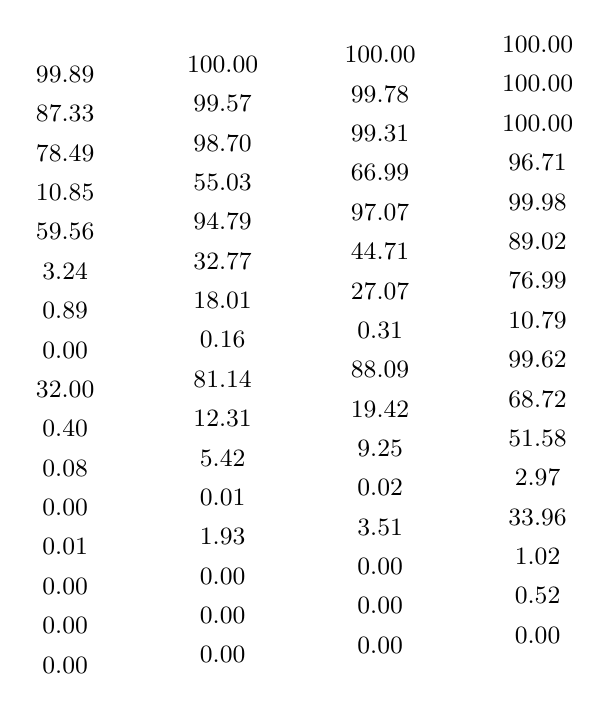
\begin{tikzpicture}
        \fontsize{9pt}{0}\selectfont
        \tree{0}{0}{6}
        \draw
            (13, 3.94) node {\BEC{100.00}}
            (11, 3.81) node {\BEC{100.00}}
            (9, 3.69) node {\BEC{100.00}}
            (7, 3.56) node {\BEC{99.89}}
            (13, 3.44) node {\BEC{100.00}}
            (11, 3.31) node {\BEC{99.78}}
            (9, 3.19) node {\BEC{99.57}}
            (7, 3.06) node {\BEC{87.33}}
            (13, 2.94) node {\BEC{100.00}}
            (11, 2.81) node {\BEC{99.31}}
            (9, 2.69) node {\BEC{98.70}}
            (7, 2.56) node {\BEC{78.49}}
            (13, 2.44) node {\BEC{96.71}}
            (11, 2.31) node {\BEC{66.99}}
            (9, 2.19) node {\BEC{55.03}}
            (7, 2.06) node {\BEC{10.85}}
            (13, 1.94) node {\BEC{99.98}}
            (11, 1.81) node {\BEC{97.07}}
            (9, 1.69) node {\BEC{94.79}}
            (7, 1.56) node {\BEC{59.56}}
            (13, 1.44) node {\BEC{89.02}}
            (11, 1.31) node {\BEC{44.71}}
            (9, 1.19) node {\BEC{32.77}}
            (7, 1.06) node {\BEC{3.24}}
            (13, 0.94) node {\BEC{76.99}}
            (11, 0.81) node {\BEC{27.07}}
            (9, 0.69) node {\BEC{18.01}}
            (7, 0.56) node {\BEC{0.89}}
            (13, 0.44) node {\BEC{10.79}}
            (11, 0.31) node {\BEC{0.31}}
            (9, 0.19) node {\BEC{0.16}}
            (7, 0.06) node {\BEC{0.00}}
            (13, -0.06) node {\BEC{99.62}}
            (11, -0.19) node {\BEC{88.09}}
            (9, -0.31) node {\BEC{81.14}}
            (7, -0.44) node {\BEC{32.00}}
            (13, -0.56) node {\BEC{68.72}}
            (11, -0.69) node {\BEC{19.42}}
            (9, -0.81) node {\BEC{12.31}}
            (7, -0.94) node {\BEC{0.40}}
            (13, -1.06) node {\BEC{51.58}}
            (11, -1.19) node {\BEC{9.25}}
            (9, -1.31) node {\BEC{5.42}}
            (7, -1.44) node {\BEC{0.08}}
            (13, -1.56) node {\BEC{2.97}}
            (11, -1.69) node {\BEC{0.02}}
            (9, -1.81) node {\BEC{0.01}}
            (7, -1.94) node {\BEC{0.00}}
            (13, -2.06) node {\BEC{33.96}}
            (11, -2.19) node {\BEC{3.51}}
            (9, -2.31) node {\BEC{1.93}}
            (7, -2.44) node {\BEC{0.01}}
            (13, -2.56) node {\BEC{1.02}}
            (11, -2.69) node {\BEC{0.00}}
            (9, -2.81) node {\BEC{0.00}}
            (7, -2.94) node {\BEC{0.00}}
            (13, -3.06) node {\BEC{0.52}}
            (11, -3.19) node {\BEC{0.00}}
            (9, -3.31) node {\BEC{0.00}}
            (7, -3.44) node {\BEC{0.00}}
            (13, -3.56) node {\BEC{0.00}}
            (11, -3.69) node {\BEC{0.00}}
            (9, -3.81) node {\BEC{0.00}}
            (7, -3.94) node {\BEC{0.00}}
        ;
    \end{tikzpicture}
\end{frame}

\begin{frame}
    \fontsize{36pt}{48pt}\selectfont
    Thm
    [Arıkan\raisebox{-9pt}{\includegraphics[height=48pt]{arikan.jpg}}]
    If, after
    \\ synthesizing $2^n$ channels,
    \\ $k$ of them are less than $p$,

    \focus<2->{polar code has rate $k/2^n$}
    \\ \focus<2->{\& block error prob $< kp$}
\end{frame}

\def\BEC#1{%
    \ifdim#1pt>99pt%
        \color{red}BEC$(#1\%)$%
    \else%
    \ifdim#1pt<1pt
        \color{teal}BEC$(#1\%)$%
    \else
        \color{gray!50!white}BEC$(#1\%)$%
    \fi
    \fi%
}

\begin{frame}
    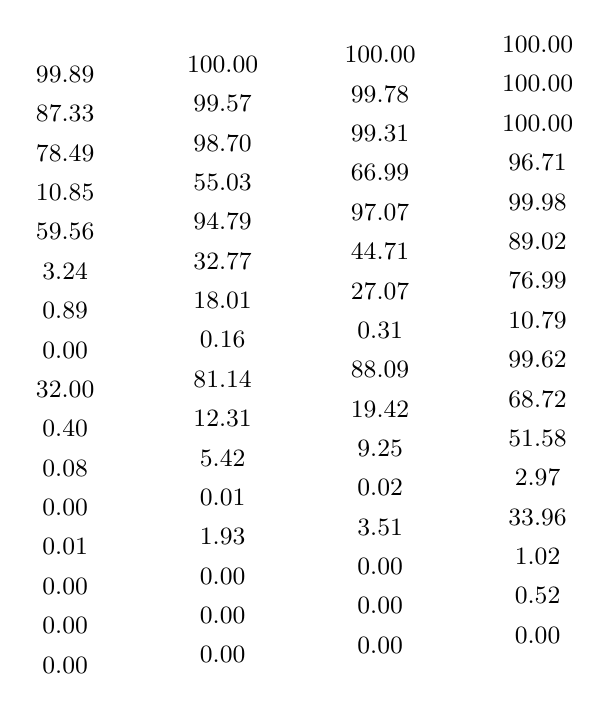
\begin{tikzpicture}
        \fontsize{9pt}{0}\selectfont
        \tree{0}{0}{6}
        \draw
            (13, 3.94) node {\BEC{100.00}}
            (11, 3.81) node {\BEC{100.00}}
            (9, 3.69) node {\BEC{100.00}}
            (7, 3.56) node {\BEC{99.89}}
            (13, 3.44) node {\BEC{100.00}}
            (11, 3.31) node {\BEC{99.78}}
            (9, 3.19) node {\BEC{99.57}}
            (7, 3.06) node {\BEC{87.33}}
            (13, 2.94) node {\BEC{100.00}}
            (11, 2.81) node {\BEC{99.31}}
            (9, 2.69) node {\BEC{98.70}}
            (7, 2.56) node {\BEC{78.49}}
            (13, 2.44) node {\BEC{96.71}}
            (11, 2.31) node {\BEC{66.99}}
            (9, 2.19) node {\BEC{55.03}}
            (7, 2.06) node {\BEC{10.85}}
            (13, 1.94) node {\BEC{99.98}}
            (11, 1.81) node {\BEC{97.07}}
            (9, 1.69) node {\BEC{94.79}}
            (7, 1.56) node {\BEC{59.56}}
            (13, 1.44) node {\BEC{89.02}}
            (11, 1.31) node {\BEC{44.71}}
            (9, 1.19) node {\BEC{32.77}}
            (7, 1.06) node {\BEC{3.24}}
            (13, 0.94) node {\BEC{76.99}}
            (11, 0.81) node {\BEC{27.07}}
            (9, 0.69) node {\BEC{18.01}}
            (7, 0.56) node {\BEC{0.89}}
            (13, 0.44) node {\BEC{10.79}}
            (11, 0.31) node {\BEC{0.31}}
            (9, 0.19) node {\BEC{0.16}}
            (7, 0.06) node {\BEC{0.00}}
            (13, -0.06) node {\BEC{99.62}}
            (11, -0.19) node {\BEC{88.09}}
            (9, -0.31) node {\BEC{81.14}}
            (7, -0.44) node {\BEC{32.00}}
            (13, -0.56) node {\BEC{68.72}}
            (11, -0.69) node {\BEC{19.42}}
            (9, -0.81) node {\BEC{12.31}}
            (7, -0.94) node {\BEC{0.40}}
            (13, -1.06) node {\BEC{51.58}}
            (11, -1.19) node {\BEC{9.25}}
            (9, -1.31) node {\BEC{5.42}}
            (7, -1.44) node {\BEC{0.08}}
            (13, -1.56) node {\BEC{2.97}}
            (11, -1.69) node {\BEC{0.02}}
            (9, -1.81) node {\BEC{0.01}}
            (7, -1.94) node {\BEC{0.00}}
            (13, -2.06) node {\BEC{33.96}}
            (11, -2.19) node {\BEC{3.51}}
            (9, -2.31) node {\BEC{1.93}}
            (7, -2.44) node {\BEC{0.01}}
            (13, -2.56) node {\BEC{1.02}}
            (11, -2.69) node {\BEC{0.00}}
            (9, -2.81) node {\BEC{0.00}}
            (7, -2.94) node {\BEC{0.00}}
            (13, -3.06) node {\BEC{0.52}}
            (11, -3.19) node {\BEC{0.00}}
            (9, -3.31) node {\BEC{0.00}}
            (7, -3.44) node {\BEC{0.00}}
            (13, -3.56) node {\BEC{0.00}}
            (11, -3.69) node {\BEC{0.00}}
            (9, -3.81) node {\BEC{0.00}}
            (7, -3.94) node {\BEC{0.00}}
        ;
    \end{tikzpicture}
\end{frame}

\def\BEC#1{%
    \ifdim#1pt>60pt%
        \color{red}BEC$(100.00\%)$
    \else%
    \ifdim#1pt<40pt%
        \color{teal}BEC$(0.00\%)$%
    \else%
        \color{gray!50!white}BEC$(#1\%)$%
    \fi
    \fi%
}

\begin{frame}
    \begin{tikzpicture}
        \fontsize{9pt}{0}\selectfont
        \tree{0}{0}{6}
        \draw
            (13, 3.94) node {\BEC{100.00}}
            (11, 3.81) node {\BEC{100.00}}
            (9, 3.69) node {\BEC{100.00}}
            (7, 3.56) node {\BEC{99.89}}
            (13, 3.44) node {\BEC{100.00}}
            (11, 3.31) node {\BEC{99.78}}
            (9, 3.19) node {\BEC{99.57}}
            (7, 3.06) node {\BEC{87.33}}
            (13, 2.94) node {\BEC{100.00}}
            (11, 2.81) node {\BEC{99.31}}
            (9, 2.69) node {\BEC{98.70}}
            (7, 2.56) node {\BEC{78.49}}
            (13, 2.44) node {\BEC{96.71}}
            (11, 2.31) node {\BEC{66.99}}
            (9, 2.19) node {\BEC{55.03}}
            (7, 2.06) node {\BEC{10.85}}
            (13, 1.94) node {\BEC{99.98}}
            (11, 1.81) node {\BEC{97.07}}
            (9, 1.69) node {\BEC{94.79}}
            (7, 1.56) node {\BEC{59.56}}
            (13, 1.44) node {\BEC{89.02}}
            (11, 1.31) node {\BEC{44.71}}
            (9, 1.19) node {\BEC{32.77}}
            (7, 1.06) node {\BEC{3.24}}
            (13, 0.94) node {\BEC{76.99}}
            (11, 0.81) node {\BEC{27.07}}
            (9, 0.69) node {\BEC{18.01}}
            (7, 0.56) node {\BEC{0.89}}
            (13, 0.44) node {\BEC{10.79}}
            (11, 0.31) node {\BEC{0.31}}
            (9, 0.19) node {\BEC{0.16}}
            (7, 0.06) node {\BEC{0.00}}
            (13, -0.06) node {\BEC{99.62}}
            (11, -0.19) node {\BEC{88.09}}
            (9, -0.31) node {\BEC{81.14}}
            (7, -0.44) node {\BEC{32.00}}
            (13, -0.56) node {\BEC{68.72}}
            (11, -0.69) node {\BEC{19.42}}
            (9, -0.81) node {\BEC{12.31}}
            (7, -0.94) node {\BEC{0.40}}
            (13, -1.06) node {\BEC{51.58}}
            (11, -1.19) node {\BEC{9.25}}
            (9, -1.31) node {\BEC{5.42}}
            (7, -1.44) node {\BEC{0.08}}
            (13, -1.56) node {\BEC{2.97}}
            (11, -1.69) node {\BEC{0.02}}
            (9, -1.81) node {\BEC{0.01}}
            (7, -1.94) node {\BEC{0.00}}
            (13, -2.06) node {\BEC{33.96}}
            (11, -2.19) node {\BEC{3.51}}
            (9, -2.31) node {\BEC{1.93}}
            (7, -2.44) node {\BEC{0.01}}
            (13, -2.56) node {\BEC{1.02}}
            (11, -2.69) node {\BEC{0.00}}
            (9, -2.81) node {\BEC{0.00}}
            (7, -2.94) node {\BEC{0.00}}
            (13, -3.06) node {\BEC{0.52}}
            (11, -3.19) node {\BEC{0.00}}
            (9, -3.31) node {\BEC{0.00}}
            (7, -3.44) node {\BEC{0.00}}
            (13, -3.56) node {\BEC{0.00}}
            (11, -3.69) node {\BEC{0.00}}
            (9, -3.81) node {\BEC{0.00}}
            (7, -3.94) node {\BEC{0.00}}
        ;
        \path <2> [overlay, opacity=0.1]
            [postaction={draw, line width=8pt}]
            [postaction={draw, line width=16pt}]
            [postaction={draw, line width=24pt}]
            (6, 0) +(-6, 0) rectangle +(6, -5)
        ;
        \draw <2> [overlay]
            (6, 0) node [below, inner sep=0]
            {\includegraphics[width=12cm]{cp.png}}
        ;
    \end{tikzpicture}
\end{frame}

\begin{frame}
    \begin{tikzpicture} [overlay]
        \fontsize{36pt}{0}\selectfont
        \draw
            (0, 0) node {\includegraphics[height=11cm]{nail.png}}
            (-0.3, -1.7) node [rotate=-20]
            {\KTV[brown!50!black][gray!50!white]{Prove polarization}}
        ;
    \end{tikzpicture}
\end{frame}

\begin{frame}
    \begin{tikzpicture} [overlay]
        \fontsize{20pt}{25pt}\selectfont
        \draw [opacity=0.2]
            (0, 0) node {\includegraphics[height=11cm]{nail.png}}
        ;
        \tikzset{xshift=-1cm, yshift=2cm}
        \draw
            (-5, 1) node [left] {$u_1$} --
            (5, 1) node [right] {BEC$(2z{-}z^2)$}
            (-5, -1) node [left] {$u_2$}  --
            (5, -1) node [right] {BEC$(z^2)$}
        ;
        \fill [CB]
            (-4.5, 1.5) rectangle node [scale=2] {\CB} (-2.5, -1.5)
        ;
        \path
            (0, 1) node [BEC] {BEC$(z)$}
            (0, -1) node [BEC] {BEC$(z)$}
        ;
        \fill [MW1] (2.5, 1.5) rectangle (4.5, -1.5) ;
        \fill [MW2]
            (2.5, 1.5) rectangle node [scale=2] {\MW} (4.5, -1.5)
        ;
        \draw
            (1, -3) node {
                \focus<2->{
                    Level$(n) \coloneqq
                    \{$the $2^n$ channels generated at level $n\}$
                }
            }
            (1, -5) node {
                \focus<3->{
                    Most BECs in Level$(n)$ are
                    BEC$(\approx1)$ or BEC$(\approx0)$
                }
            }
        ;
    \end{tikzpicture}
\end{frame}

\begin{frame}
    \begin{tikzpicture} [overlay]
        \fontsize{30pt}{40pt}\selectfont
        \draw
            (0, 0) node [rotate=30]
            {\includegraphics[height=11cm]{hammer.png}}
            (3, 0.5) node [rotate=-30]
            {\KTV[brown][gray]{Jensen's inequality}}
        ;
    \end{tikzpicture}
\end{frame}

\begin{frame}
    \begin{tikzpicture} [overlay]
        \fontsize{20pt}{0}\selectfont
        \draw
            (0, 0) node {\includegraphics[width=16cm]{bliss.jpg}}
            (8, -4.5) node [above left]
            {\fontsize{6pt}{0}\selectfont\color{gray}ChatGPT}
        ;
        \fill
            (0, 2.3) circle (5pt) node [above] {$(z, h(z))$}
            (-4, 1.2) circle (5pt) node [above] {$(z^2, h(z^2))$}
            (4, 0.1) circle (5pt) node [below]
            {\KTV[white][black]{$(2z-z^2, h(2z-z^2))$}}
        ;
        \draw <2-> (-4, 1.2) -- (4, 0.1);
        \fill <2-> (0, 0.6) circle (5pt) node [below] {avg};
        \draw <3-> (0, -3) node{
            $\displaystyle \frac1{2^n} \sum_{z\in\text{Level}(n)} h(z)$
            \KTV[white][black]{decreases as $n \to \infty$}
        };
    \end{tikzpicture}
\end{frame}

\begin{frame}
    \begin{tikzpicture} [overlay]
        \fontsize{20pt}{0}\selectfont
        \draw [opacity=0.3]
            (0, 0) node {\includegraphics[width=16cm]{bliss.jpg}}
        ;
        \draw (-5, 0) node [align=center] {
            \includegraphics[width=4cm]{nail.png}
            \\ Prove polarization
        };
        \draw <2-> (0, 0) node [align=center] {
            \includegraphics[width=4cm]{hammer.png}
            \\ Jensen's
        };
        \draw <3-> (5, 0) node [align=center] {
            \includegraphics[width=4cm]{nail.png}
            \\ Convex function?
        };
    \end{tikzpicture}
\end{frame}

\begin{frame}
    \begin{tikzpicture} [overlay]
        \fontsize{20pt}{0}\selectfont
        \draw [opacity=0.3]
            (0, 0) node {\includegraphics[width=16cm]{bliss.jpg}}
        ;
        \draw
            (0, 3) node{
                Hill shape
                $h(z) \coloneqq \bigl(z (1 - z)\bigr)^{0.663}$
                % $h(z) \coloneqq \bigl(z (1 - z)\bigr)^{0.72427}$
            }
            (0, 0) node [align=center] {
                \focus<2->{
                    $\displaystyle \sup_{0<z<1}
                    \frac{h(z^2) + h(2z - z^2)}{2h(z)}
                    < 0.832$
                }
            }
            (0, -3) node [align=center] {
                \focus<3->{
                    $\displaystyle \frac1{2^n}
                    \sum_{z\in\text{Level}(n)} h(z) < 0.832^n$
                }
            }
        ;
        \pgfmathsetseed{20240124}
        \draw <4->
            (0, 2.3) node {\TV}
            (-4, 1.2) node {\TV}
            (2, 1.3) node {\TV}
            foreach \j in {1, ..., 20} {
                (-8, -3) +([rotate=45] rnd*2.5, rand/2) node {\TV}
                (8, -3) +([rotate=135] rnd*2.5, rand/2) node {\TV}
            }
        ;
    \end{tikzpicture}
\end{frame}

\begin{frame}
    \begin{tikzpicture} [overlay]
        \fontsize{16pt}{0}\selectfont
        \draw [opacity=0.3]
            (0, 0) node {\includegraphics[width=16cm]{bliss.jpg}}
        ;
        \draw (-5, 0) node [align=center] {
            \includegraphics[width=4cm]{nail.png}
            \\ Prove polarization
        };
        \draw <2-> (-2, 0) node [align=center] {
            \includegraphics[width=4cm]{hammer.png}
            \\ Jensen's
        };
        \draw <3-> (2, 0) node [align=center] {
            \includegraphics[width=4cm]{nail.png}
            \\ Convex function?
        };
        \draw <4-> (5, 0) node [align=center] {
            \includegraphics[width=4cm]{hammer.png}
            \\ $\bigl(z (1 - z)\bigr)^{0.663}$
        };
    \end{tikzpicture}
\end{frame}

\begin{frame}
    \fontsize{36pt}{48pt}\selectfont
    \begin{tikzpicture} [overlay, opacity=0.5]
        \draw <3-> (1.5, -1) node {
            \includegraphics[height=6cm]{stretch.jpg}%
            \llap{\fontsize{6pt}{0}\selectfont\color{gray}ChatGPT}%
        };
    \end{tikzpicture}%
    If $k$ of $2^n$ are less than $p$,
    polar code has rate $k/2^n$
    \\ \& block error prob $< kp$.

    \focus<2->{$k/2^n = 60\% - 2^{-\Omega(n)}$}
    \\ \focus<2->{$p = 2^{-\Omega(n)}$}
\end{frame}

\begin{frame}
    \begin{tikzpicture} [overlay]
        \fontsize{36pt}{0}\selectfont
        \draw
            (0, 0) node {\includegraphics[height=11cm]{nail.png}}
            (-0.3, -1.7) node [rotate=-20]
            {\KTV[brown!50!black][gray!50!white]{Let's improve $p$}}
        ;
    \end{tikzpicture}
\end{frame}

\begin{frame}
    \begin{tikzpicture} [overlay]
        \fontsize{20pt}{25pt}\selectfont
        \draw [opacity=0.2]
            (0, 0) node {\includegraphics[height=11cm]{nail.png}}
        ;
        \tikzset{xshift=-1cm, yshift=2cm}
        \draw
            (-5, 1) node [left] {$u_1$} --
            (5, 1) node [right] {BEC$(2z{-}z^2)$}
            (-5, -1) node [left] {$u_2$}  --
            (5, -1) node [right] {BEC$(z^2)$}
        ;
        \fill [CB]
            (-4.5, 1.5) rectangle node [scale=2] {\CB} (-2.5, -1.5)
        ;
        \path
            (0, 1) node [BEC] {BEC$(z)$}
            (0, -1) node [BEC] {BEC$(z)$}
        ;
        \fill [MW1] (2.5, 1.5) rectangle (4.5, -1.5) ;
        \fill [MW2]
            (2.5, 1.5) rectangle node [scale=2] {\MW} (4.5, -1.5)
        ;
    \end{tikzpicture}
\end{frame}

\def\beciter#1#2#3{%z, depth, depth left
    \ifnum#3>0
        \pgfmathtruncatemacro\a{#2}
        \pgfmathtruncatemacro\b{\a+1}
        \pgfmathtruncatemacro\c{#3}
        \pgfmathtruncatemacro\d{\c-1}
        \pgfmathsetmacro\y{#1}
        \pgfmathsetmacro\ychange{\y*(10-\y)/10}
        \pgfmathsetmacro\yup{\y+\ychange}
        \pgfmathsetmacro\ydown{\y-\ychange}
        \draw
            (\a, \y) -- (\b, \yup)
            (\a, \y) -- (\b, \ydown)
        ;
        \ifnum#2<5
            \draw
                (\a, \y) node [fill=yellow!80!black, inner sep=0] {\MW}
            ;
        \fi
        {\beciter{\yup}{\b}{\d}}
        {\beciter{\ydown}{\b}{\d}}
    \fi
}

\begin{frame}
    \begin{tikzpicture} [overlay]
        \fontsize{20pt}{25pt}\selectfont
        \draw [opacity=0.2]
            (0, 0) node {\includegraphics[height=11cm]{nail.png}}
        ;
        \tikzset{xshift=-1cm, yshift=2cm}
        \draw
            (-5, 1) node [left] {$u_1$} --
            (5, 1) node [right] {BEC$(2z{-}z^2)$}
            (-5, -1) node [left] {$u_2$}  --
            (5, -1) node [right] {BEC$(z^2)$}
        ;
        \fill [CB]
            (-4.5, 1.5) rectangle node [scale=2] {\CB} (-2.5, -1.5)
        ;
        \path
            (0, 1) node [BEC] {BEC$(z)$}
            (0, -1) node [BEC] {BEC$(z)$}
        ;
        \fill [MW1] (2.5, 1.5) rectangle (4.5, -1.5) ;
        \fill [MW2]
            (2.5, 1.5) rectangle node [scale=2] {\MW} (4.5, -1.5)
        ;
        \tikzset{xshift=-6.5cm, yshift=-6cm, yscale=0.8, xscale=1.8}
        \only<2>{
            \fill [white, overlay] (0, -10) rectangle (1, 10);
            \beciter{4}{0}{1}
        }
        \only<3>{
            \fill [white, overlay] (0, -10) rectangle (2, 10);
            \beciter{4}{0}{2}
        }
        \only<4>{
            \fill [white, overlay] (0, -10) rectangle (3, 10);
            \beciter{4}{0}{3}
        }
        \only<5>{
            \fill [white, overlay] (0, -10) rectangle (4, 10);
            \beciter{4}{0}{4}
        }
        \only<6>{
            \fill [white, overlay] (0, -10) rectangle (5, 10);
            \beciter{4}{0}{5}
        }
        \only<7>{
            \fill [white, overlay] (0, -10) rectangle (6, 10);
            \beciter{4}{0}{6}
        }
        \only<8>{
            \fill [white, overlay] (0, -10) rectangle (7, 10);
            \beciter{4}{0}{7}
        }
        \only<9>{
            \fill [white, overlay] (0, -10) rectangle (8, 10);
            \beciter{4}{0}{8}
        }
        \draw [->] (0, 0) -- (0, 10) node [right] {$z$};
        \draw [->] (0, 0) -- (8.5, 0) node [above] {$n$};
    \end{tikzpicture}
\end{frame}

\begin{frame}
    
\begin{tikzpicture} [overlay]
        \fontsize{20pt}{25pt}\selectfont
        \tikzset{xshift=-7.5cm, yshift=-4cm, yscale=0.8, xscale=1.8}
        \beciter{4}{0}{8}
        \draw [->] (0, 0) -- (0, 10) node [right] {$z$};
        \draw [->] (0, 0) -- (8.5, 0) node [above] {$n$};
        \draw [red, line width=4pt, fill=white, opacity=0.9]
            (4, 9) rectangle (10, 1)
            (4, 5) node [right, align=center] {Level \\ $n/2$}
        ;
        \draw [red]
            (6, 9) node [below] {\focus<2->{$z = 1 - 2^{-\Omega(n/2)}$}}
            (6, 1) node [above] {\focus<2->{$z = 2^{-\Omega(n/2)}$}}
            (7, 5) node [align=center] {
                \focus<3->{$2^{-\Omega(n/2)}$ fraction}
                \\ \focus<3->{of channels}
                \\ \focus<3->{have been here}
            }
        ;
        \draw <4> [teal, line width=4pt, fill=white, opacity=0.9,
            rounded corners=24pt]
            (0.5, 8) rectangle node [align=center] {
                These channels,
                \\ most of them
                \\ (Hoeffding)
                \\ undergo $z \mapsto z^2$
                \\ $n/5$ times
            } (3.5, 1)
            (3, 1) edge [->, out=-90, in=180] (4, 0.5) 
        ;
        \draw <5-> [teal, line width=4pt, fill=white, opacity=0.9,
            rounded corners=24pt]
            (0.5, 8) rectangle node [align=center] {
                Squaring
                \\ $n/5$ times
                \\ make $z$
                \\ $(2^{-\Omega(n/2)})^{2^{n/5}}$
                \\ \focus<6>{$< 2^{-2^{n/5}}$}
            } (3.5, 1)
            (3, 1) edge [->, out=-90, in=180] (4, 0.5) 
        ;
    \end{tikzpicture}
\end{frame}

\begin{frame}
    \fontsize{36pt}{48pt}\selectfont
    If $k$ of $2^n$ are less than $p$,
    polar code has rate $k/2^n$
    \\ \& block error prob $< kp$.

    $k/2^n = 60\% - 2^{-\Omega(n)}$
    \\
    \tikz [baseline=(X.base)]
    \draw[red] node (X) {$p = 2^{-\Omega(n)}$} (X.200) -- (X.20);
    \color{teal} $p = 2^{-2^{\Omega(n)}}$
\end{frame}

\begin{frame}
    \begin{tikzpicture} [overlay, yshift=0.5cm]
        \draw (-5, 2) node [align=center] {
            \includegraphics[width=4cm]{nail.png}
            \\ Prove polarization
        };
        \draw <2-> (-2, 2) node [align=center] {
            \includegraphics[width=4cm]{hammer.png}
            \\ Jensen's
        };
        \draw <3-> (2, 2) node [align=center] {
            \includegraphics[width=4cm]{nail.png}
            \\ Convex function?
        };
        \draw <4-> (5, 2) node [align=center] {
            \includegraphics[width=4cm]{hammer.png}
            \\ $\bigl(z (1 - z)\bigr)^{0.663}$
        };
        \draw <5-> (-5, -2) node [align=center] {
            \includegraphics[width=4cm]{nail.png}
            \\ $p$ too bad
        };
        \draw <6-> (-2, -2) node [align=center] {
            \includegraphics[width=4cm]{hammer.png}
            \\ Hoeffding $p$
        };
        \draw <7-> (2, -2) node [align=center] {
            \includegraphics[width=4cm]{nail.png}
            \\ Improvements
        };
        \draw <7-> (6, -2) node [align=center] {
            \includegraphics[width=4cm]{nail.png}
            \\ Generalizations
        };
    \end{tikzpicture}
\end{frame}

\begin{frame}
    \begin{tikzpicture} [overlay, yshift=0.3cm]
        \fontsize{12pt}{16pt}\selectfont
        \draw (0, 0) node {
            \includegraphics[height=9cm]{hands.jpg}%
            \llap{\fontsize{6pt}{0}\selectfont\color{gray}ChatGPT}%
        };
        \draw <2->
            (-1.5, -2.5) node [align=center] {
                \KTV[white][gray]{successive}
                \\ \KTV[white][gray]{cancellation}
            }
            (1.5, -2.5) node [align=center] {
                \KTV[white][gray]{channel}
                \\ \KTV[white][gray]{polarization}
            }
        ;
        \draw <3->
            (-1.5, -0.5) node [align=center] {
                \KTV[white][black]{better gap}
                \\ \KTV[white][black]{to capacity}
            }
            (1.5, -0.5) node [align=center] {
                \KTV[white][black]{better}
                \\ \KTV[white][black]{error prob}
            }
        ;
        \draw <4->
            (-1, 3.7) node [left] {large matrix/RS/AG}
            (1, 3.7) node [right] {BMS/large alphabet}
        ;
        \draw <5->
            (-3, 2) node [left] {MAC/broadcast/wiretap}
            (3, 2) node [right] {lossy/distribut compress}
        ;
        \draw <6->
            (-4, 0.3) node [left] {classical--quantum}
            (4, 0.3) node [right] {insdel channel}
        ;
        \draw <7->
            (-3.5, -1.5) node [left] {coded computation}
            (3.5, -1.5) node [right] {PAC \& list decoding}
        ;
    \end{tikzpicture}
\end{frame}

\begin{frame}
    \begin{tikzpicture} [overlay, yshift=0.3cm]
        \fontsize{12pt}{16pt}\selectfont
        \draw (0, 0) node {
            \includegraphics[height=9cm]{hands.jpg}%
            \llap{\fontsize{6pt}{0}\selectfont\color{gray}ChatGPT}%
        };
        \draw
            (-1.5, -2.5) node [align=center] {
                \KTV[white][gray]{successive}
                \\ \KTV[white][gray]{cancellation}
            }
            (1.5, -2.5) node [align=center] {
                \KTV[white][gray]{channel}
                \\ \KTV[white][gray]{polarization}
            }
            (-1.5, -0.5) node [align=center] {
                \KTV[white][black]{better gap}
                \\ \KTV[white][black]{to capacity}
            }
            (1.5, -0.5) node [align=center] {
                \KTV[white][black]{better}
                \\ \KTV[white][black]{error prob}
            }
            (-1, 3.7) node [left] {large matrix/RS/AG}
            (1, 3.7) node [right] {BMS/large alphabet}
            (-3, 2) node [left] {MAC/broadcast/wiretap}
            (3, 2) node [right] {lossy/distribut compress}
            (-4, 0.3) node [left] {classical--quantum}
            (4, 0.3) node [right] {insdel channel}
            (-3.5, -1.5) node [left] {coded computation}
            (3.5, -1.5) node [right] {PAC \& list decoding}
        ;
        \fill [gray!50!white, opacity=0.7, even odd rule]
            (0, 0) circle (10) (-1.5, -0.5) circle (2)
        ;
    \end{tikzpicture}
\end{frame}

\begin{frame}
    \begin{tikzpicture} [overlay]
        \fontsize{20pt}{0}\selectfont
        \draw [opacity=0.3]
            (0, 0) node {\includegraphics[width=16cm]{bliss.jpg}}
        ;
        \draw
            (0, 3) node{
                Hill shape
                $h(z) \coloneqq \bigl(z (1 - z)\bigr)^{0.663}$
                % $h(z) \coloneqq \bigl(z (1 - z)\bigr)^{0.72427}$
                is not optimal
            }
            (0, 0) node [align=center] {
                $\displaystyle \sup_{0<z<1}
                \frac{h(z^2) + h(2z - z^2)}{2h(z)}
                < 0.832$
            }
            (0, -3) node [align=center] {
                \focus<2->{
                    Use power method
                    $\displaystyle h_{i+1}(z) \coloneqq
                    \frac{h_i(z^2) + h_i(2z - z^2)}{\text{normalize}}$
                }
            }
        ;
        \draw <3-> (5, 0) node {
            \includegraphics[height=3cm]{nail_text.png}
        };
    \end{tikzpicture}
\end{frame}

\begin{frame}
    \begin{tikzpicture} [overlay, yshift=0.3cm]
        \fontsize{12pt}{16pt}\selectfont
        \draw (0, 0) node {
            \includegraphics[height=9cm]{hands.jpg}%
            \llap{\fontsize{6pt}{0}\selectfont\color{gray}ChatGPT}%
        };
        \draw
            (-1.5, -2.5) node [align=center] {
                \KTV[white][gray]{successive}
                \\ \KTV[white][gray]{cancellation}
            }
            (1.5, -2.5) node [align=center] {
                \KTV[white][gray]{channel}
                \\ \KTV[white][gray]{polarization}
            }
            (-1.5, -0.5) node [align=center] {
                \KTV[white][black]{better gap}
                \\ \KTV[white][black]{to capacity}
            }
            (1.5, -0.5) node [align=center] {
                \KTV[white][black]{better}
                \\ \KTV[white][black]{error prob}
            }
            (-1, 3.7) node [left] {large matrix/RS/AG}
            (1, 3.7) node [right] {BMS/large alphabet}
            (-3, 2) node [left] {MAC/broadcast/wiretap}
            (3, 2) node [right] {lossy/distribut compress}
            (-4, 0.3) node [left] {classical--quantum}
            (4, 0.3) node [right] {insdel channel}
            (-3.5, -1.5) node [left] {coded computation}
            (3.5, -1.5) node [right] {PAC \& list decoding}
        ;
        \fill [gray!50!white, opacity=0.7, even odd rule]
            (0, 0) circle (10) (1.5, -0.5) circle (2)
        ;
    \end{tikzpicture}
\end{frame}

\begin{frame}
    \begin{tikzpicture} [overlay]
        \fontsize{20pt}{25pt}\selectfont
        \tikzset{xshift=-7.5cm, yshift=-4cm, yscale=0.8, xscale=1.8}
        \beciter{4}{0}{8}
        \draw [->] (0, 0) -- (0, 10) node [right] {$z$};
        \draw [->] (0, 0) -- (8.5, 0) node [above] {$n$};
        \draw [red, line width=4pt, fill=white, opacity=0.9]
            (4, 9) rectangle (10, 1)
            (4, 5) node [right, align=center] {Level \\ $n/2$}
        ;
        \draw [red]
            (6, 9) node [below] {\strut{$z = 1 - 2^{-\Omega(n/2)}$}}
            (6, 1) node [above] {\strut{$z = 2^{-\Omega(n/2)}$}}
            (7, 5) node [align=center] {
                \strut{$2^{-\Omega(n/2)}$ fraction}
                \\ \strut{of channels}
                \\ \strut{have been here}
            }
        ;
        \draw [teal, line width=4pt, fill=white, opacity=0.9,
            rounded corners=24pt]
            (0.5, 8) rectangle node [align=center] {
                These channels,
                \\ most of them
                \\ (Hoeffding)
                \\ undergo $z \mapsto z^2$
                \\ $n/5$ times
            } (3.5, 1)
            (3, 1) edge [->, out=-90, in=180] (4, 0.5) 
        ;
    \end{tikzpicture}
\end{frame}

\begin{frame}
    \begin{tikzpicture} [overlay]
        \fontsize{20pt}{25pt}\selectfont
        \tikzset{xshift=-7.5cm, yshift=-4cm, yscale=0.8, xscale=1.8}
        \beciter{4}{0}{8}
        \draw [->] (0, 0) -- (0, 10) node [right] {$z$};
        \draw [->] (0, 0) -- (8.5, 0) node [above] {$n$};
        \draw [red, line width=4pt, fill=white, opacity=0.9]
            (3, 9) rectangle (10, 1)
            (3, 5) node [right, align=center] {Level \\ $n/3$}
        ;
        \draw [red]
            (6, 9) node [below] {\focus<2->{$z = 1 - 2^{-\Omega(n/3)}$}}
            (6, 1) node [above] {\focus<2->{$z = 2^{-\Omega(n/3)}$}}
            (7, 5) node [align=center] {
                \focus<3->{$2^{-\Omega(n/3)}$ fraction}
                \\ \focus<3->{of channels}
                \\ \focus<3->{have been here}
            }
        ;
        \draw <4-> [teal, line width=4pt, fill=white, opacity=0.9,
            rounded corners=24pt]
            (0.5, 8) rectangle node [align=center] {
                These channels,
                \\ most of them
                \\ (Hoeffding)
                \\ undergo $z \mapsto z^2$
                \\ $(1/3 - \varepsilon) n$ times
            } (3.5, 1)
            (3, 1) edge [->, out=-90, in=180] (4, 0.5) 
        ;
    \end{tikzpicture}
\end{frame}

\begin{frame}
    \fontsize{36pt}{48pt}\selectfont
    If $k$ of $2^n$ are less than $p$,
    polar code has rate $k/2^n$
    \\ \& block error prob $< kp$.

    $k/2^n = 60\% - 2^{-n/3.627}$
    \\
    $p = 2^{-2^{\Omega(n)}}$
\end{frame}

\begin{frame}
    \fontsize{36pt}{48pt}\selectfont
    If $k$ of $2^n$ are less than $p$,
    polar code has rate $k/2^n$
    \\ \& block error prob $< kp$.

    $k/2^n = 60\% - 2^{-\delta n}$
    \\
    $p = 2^{-2^{(1/2-\varepsilon)n}}$
\end{frame}

\begin{frame}
    \includegraphics[width=15.5cm]{hypotenuse.png}

    $\rho =$ exponent in gap; $pi$ = exponent in error
\end{frame}

\begin{frame}
    \includegraphics[height=8cm]{en23.png}
\end{frame}

\begin{frame}
    \fontsize{36pt}{48pt}\selectfont
    If $k$ of $2^n$ are less than $p$,
    polar code has rate $k/2^n$
    \\ \& block error prob $< kp$.

    $k/2^n = 60\% - 2^{-n/3.627}$
    \\
    $p = 2^{-2^{\Omega(n)}}$
\end{frame}

\begin{frame}
    \includegraphics[height=8cm]{een13.png}
\end{frame}


\begin{frame}
    \includegraphics[width=15.5cm]{hypotenuse.png}
\end{frame}

\begin{frame}
    \begin{tikzpicture} [overlay, yshift=0.3cm]
        \fontsize{12pt}{16pt}\selectfont
        \draw (0, 0) node {
            \includegraphics[height=9cm]{hands.jpg}%
            \llap{\fontsize{6pt}{0}\selectfont\color{gray}ChatGPT}%
        };
        \draw
            (-1.5, -2.5) node [align=center] {
                \KTV[white][gray]{successive}
                \\ \KTV[white][gray]{cancellation}
            }
            (1.5, -2.5) node [align=center] {
                \KTV[white][gray]{channel}
                \\ \KTV[white][gray]{polarization}
            }
            (-1.5, -0.5) node [align=center] {
                \KTV[white][black]{better gap}
                \\ \KTV[white][black]{to capacity}
            }
            (1.5, -0.5) node [align=center] {
                \KTV[white][black]{better}
                \\ \KTV[white][black]{error prob}
            }
            (-1, 3.7) node [left] {large matrix/RS/AG}
            (1, 3.7) node [right] {BMS/large alphabet}
            (-3, 2) node [left] {MAC/broadcast/wiretap}
            (3, 2) node [right] {lossy/distribut compress}
            (-4, 0.3) node [left] {classical--quantum}
            (4, 0.3) node [right] {insdel channel}
            (-3.5, -1.5) node [left] {coded computation}
            (3.5, -1.5) node [right] {PAC \& list decoding}
        ;
        \fill [gray!50!white, opacity=0.7]
            (0, 0) -- (100 : 10) arc (100 : -210 : 10) -- (0, 0)
        ;
    \end{tikzpicture}
\end{frame}

\begin{frame}
    \begin{tikzpicture}
        \fontsize{20pt}{25pt}\selectfont
        \draw
            (-5, -1) node [left] {$u_1$} --
            (5, -1) node [right] {BEC$(2z - z^2)$}
            (-5, -3) node [left] {$u_2$}  --
            (5, -3) node [right] {BEC$(z^2)$}
        ;
        \fill [CB]
            (-4.5, -0.5) rectangle node [scale=2] {\CB} (-2.5, -3.5)
        ;
        \path
            (0, -1) node [BEC] {BEC$(z)$}
            (0, -3) node [BEC] {BEC$(z)$}
        ;
        \fill [MW1] (2.5, -0.5) rectangle (4.5, -3.5);
        \fill [MW2]
            (2.5, -0.5) rectangle node [scale=2] {\MW} (4.5, -3.5)
        ;
        \draw
            (0, -5) node [shading=color wheel] {
                \KTV[black][white]{Upgrade \emoji{gem-stone}x4}
            }
        ;
    \end{tikzpicture}
\end{frame}

\begin{frame}
    \begin{tikzpicture}
        \fontsize{20pt}{25pt}\selectfont
        \draw
            (-5, -1) node [left] {$u_1$} --
            (5, -1) node [right] {BEC$(3z{-}3z^2{+}z^3)$}
            (-5, -3) node [left] {$u_2$}  --
            (5, -3) node [right] {BEC$(2z^2 - z^3)$}
            (-5, -5) node [left] {$u_3$}  --
            (5, -5) node [right] {BEC$(z^2)$}
        ;
        \fill [CB]
            (-4.5, -0.5) rectangle node [scale=2] {\CB} (-2.5, -5.5)
        ;
        \path
            (0, -1) node [BEC] {BEC$(z)$}
            (0, -3) node [BEC] {BEC$(z)$}
            (0, -5) node [BEC] {BEC$(z)$}
        ;
        \fill [MW1] (2.5, -0.5) rectangle (4.5, -5.5) ;
        \fill [MW2]
            (2.5, -0.5) rectangle node [scale=2] {\MW} (4.5, -5.5)
        ;
        \draw
            (0, -7) node [shading=color wheel] {
                \KTV[black][white]{Upgrade \emoji{gem-stone}x8}
            }
        ;
    \end{tikzpicture}
\end{frame}

\begin{frame}
    \begin{tikzpicture} [yscale=0.9]
        \fontsize{20pt}{25pt}\selectfont
        \draw
            (-5, -1) node [left] {$u_1$} --
            (5, -1) node [right] {BEC$(f_1(z))$}
            (-5, -3) node [left] {$u_2$}  --
            (5, -3) node [right] {BEC$(f_2(z))$}
            (-5, -5) node [left] {$u_3$}  --
            (5, -5) node [right] {BEC$(f_3(z))$}
            (-5, -7) node [left] {$u_4$}  --
            (5, -7) node [right] {BEC$(f_4(z))$}
        ;
        \fill [CB]
            (-4.5, -0.5) rectangle node [scale=2] {\CB} (-2.5, -7.5)
        ;
        \path
            (0, -1) node [BEC] {BEC$(z)$}
            (0, -3) node [BEC] {BEC$(z)$}
            (0, -5) node [BEC] {BEC$(z)$}
            (0, -7) node [BEC] {BEC$(z)$}
        ;
        \fill [MW1] (2.5, -0.5) rectangle (4.5, -7.5) ;
        \fill [MW2]
            (2.5, -0.5) rectangle node [scale=2] {\MW} (4.5, -7.5)
        ;
        \draw
            (0, -9) node [shading=color wheel] {
                \KTV[black][white]{Upgrade \emoji{gem-stone}x16}
            }
        ;
    \end{tikzpicture}
\end{frame}

\begin{frame}
    \begin{tikzpicture} [yscale=0.75]
        \fontsize{20pt}{25pt}\selectfont
        \draw
            (-5, -1) node [left] {$u_1$} --
            (5, -1) node [right] {BEC$(f_1(z))$}
            (-5, -3) node [left] {$u_2$}  --
            (5, -3) node [right] {BEC$(f_2(z))$}
            (-5, -5) node [left] {$u_3$}  --
            (5, -5) node [right] {BEC$(f_3(z))$}
            (-5, -7) node [left] {$u_4$}  --
            (5, -7) node [right] {BEC$(f_4(z))$}
            (-5, -9) node [left] {$u_5$}  --
            (5, -9) node [right] {BEC$(f_5(z))$}
        ;
        \fill [CB]
            (-4.5, -0.5) rectangle node [scale=2] {\CB} (-2.5, -9.5)
        ;
        \path
            (0, -1) node [BEC] {BEC$(z)$}
            (0, -3) node [BEC] {BEC$(z)$}
            (0, -5) node [BEC] {BEC$(z)$}
            (0, -7) node [BEC] {BEC$(z)$}
            (0, -9) node [BEC] {BEC$(z)$}
        ;
        \fill [MW1] (2.5, -0.5) rectangle (4.5, -9.5) ;
        \fill [MW2]
            (2.5, -0.5) rectangle node [scale=2] {\MW} (4.5, -9.5)
        ;
        \draw
            (0, -11) node [shading=color wheel] {
                \KTV[black][white]{Upgrade \emoji{gem-stone}x32}
            }
        ;
    \end{tikzpicture}
\end{frame}

\begin{frame}
    \fontsize{20pt}{28pt}\selectfont
    \raisebox{-10pt}{\scalebox{2}{\CB}}
    $= \ell \times \ell$ matrices such as
    \scalebox{0.2}{$\begin{bmatrix}
        1
        \\1&1
        \\1&&1
        \\1&&&&1
        \\1&1&1&1
        \\1&1&&&1&1
        \\1&&1&&1&&1
        \\1&1&1&1&1&1&1&1
    \end{bmatrix}$}

    \vfill\pause

    $X_1^\ell \coloneqq U_1^\ell$\CB

    $Y_1^\ell \coloneqq$ channel output of $X_1^j$

    The $j$th new-channel is $(U_j|Y_1^\ell U_1^{j-1})$

    \vfill\pause

    $\displaystyle f_j(z) \coloneqq
    \sum_{C\subset\text{columns}(\text{\CB})}
    \bigl(\operatorname{rk}(C_{j-1}){-}\operatorname{rk}(C_j)\bigr)
    z^{\ell-|C|} (1{-}z)^{|C|}$
    \\ where $C_j$ is $C$ with first $j$ rows removed
\end{frame}

\begin{frame}
    \begin{tikzpicture} [overlay]
        \fontsize{20pt}{0}\selectfont
        \draw
            (0, 0) node {\includegraphics[width=16cm]{bliss.jpg}}
            (8, -4.5) node [above left]
            {\fontsize{6pt}{0}\selectfont\color{gray}ChatGPT}
        ;
        \fill
            (0, 2.3) circle (5pt) node [above] {$(z, h(z))$}
            (-5, 0.2) circle (5pt) node [below] {$(f_1(z), h(f_1(z)))$}
            (-4, 1.2) circle (5pt) node [above] {$(f_2(z), h(f_2(z)))$}
            (1, 1.9) circle (5pt) node [right] {$(f_3(z), h(f_3(z)))$}
            (3, 0.8) circle (5pt) node [below] {$(f_4(z), h(f_4(z)))$}
            (5, -0.7) circle (5pt) node [below] {$(f_5(z), h(f_5(z)))$}
        ;
        \draw <2-> (0, -3) node{
            Upper bound
            \KTV[white][black]{
                $\displaystyle \sup_{0<z<1}\frac1{5h(z)}
                \sum_{j=1}^5 h(f_j(z))$
        }
        };
    \end{tikzpicture}
\end{frame}

\def\murange#1#2{\tikz[x=8cm]{
	\draw [teal] (0, 0) -- (1/2, 0);
	\draw [Parenthesis-Parenthesis, line width=2pt]
        (#1, 0) -- (#2, 0)
    ;
}}
\def\mupoint#1{\tikz[x=8cm]{
	\draw [teal] (0, 0) -- (1/2, 0);
	\fill (#1, 0) circle [radius=.2em];
}}

\begin{frame}
    \fontsize{20pt}{0}\selectfont
    Gap to capacity $= \dfrac1{\text{block length}^{???}}$ over BEC   \\
    \fontsize{12pt}{24pt}\selectfont
    \raggedleft \rightskip1cm
    \pause           \hfill\hbox to4cm{\color{teal} $0$ \hfill $1/2$} \\
    2010 Hassani--Alishahi--Urbanke    $2 \times 2$ \mupoint{1/3.627} \\
    2010 Korada--Montanari--Telatar--Urbanke
                                       $2 \times 2$ \mupoint{1/3.627} \\
    \pause
    2014 Fazeli--Vardy                 $8 \times 8$ \mupoint{1/3.577} \\
    \pause
    2021 Trofimiuk--Trifonov         $16 \times 16$ \mupoint{1/3.346} \\
    \focus<5->
    {2022 Duursma--Gabrys--Guruswami--Lin--W \CB $\in F_4^{2\times2}$}
                                                    \mupoint{1/3.328} \\
    2021 Trofimiuk                   $24 \times 24$ \mupoint{1/3.308} \\
    2021 Yao--Fazeli--Vardy          $32 \times 32$ \mupoint{1/3.122} \\
    2021 Yao--Fazeli--Vardy           $64 \times 64$ \mupoint{1/2.87} \\
\end{frame}

\begin{frame}
    \begin{tikzpicture}
        \fontsize{20pt}{25pt}\selectfont
        \draw
            (-5, -1) node [left] {$u_1$} --
            (5, -1) node [right] {BEC$(2z - z^2)$}
            (-5, -3) node [left] {$u_2$}  --
            (5, -3) node [right] {BEC$(z^2)$}
        ;
        \fill [CB]
            (-4.5, -0.5) rectangle node [scale=2] {\CB} (-2.5, -3.5)
        ;
        \path
            (0, -1) node [BEC] {BEC$(z)$}
            (0, -3) node [BEC] {BEC$(z)$}
        ;
        \fill [MW1] (2.5, -0.5) rectangle (4.5, -3.5);
        \fill [MW2]
            (2.5, -0.5) rectangle node [scale=2] {\MW} (4.5, -3.5)
        ;
        \draw
            (0, -5) node [shading=color wheel] {
                \KTV[black][white]{Upgrade \emoji{gem-stone}x1}
            }
        ;
    \end{tikzpicture}
\end{frame}

\begin{frame}
    \begin{tikzpicture}
        \fontsize{20pt}{25pt}\selectfont
        \tikzset{BEC/.style={
            draw=cyan!50!black, fill=cyan!50!white, rounded corners=6pt,
        }}
        \draw [double, double distance=0.1cm, line cap=butt]
            (-5, -1) node [left] {$u_1u_2$} --
            (5, -1) node [right] {TetraEC}
            (-5, -3) node [left] {$u_3u_4$}  --
            (5, -3) node [right] {TetraEC}
        ;
        \fill [CB]
            (-4.5, -0.5) rectangle
            node [black] {$F_4^{2\times2}$} (-2.5, -3.5)
        ;
        \path
            (0, -1) +(-0.1, -0.1) node [BEC] {BEC$(z)^2$}
            (0, -1) +(0.1, 0.1) node [BEC] {BEC$(z)^2$}
            (0, -3) +(-0.1, -0.1) node [BEC] {BEC$(z)^2$}
            (0, -3) +(0.1, 0.1) node [BEC] {BEC$(z)^2$}
        ;
        \fill [MW1] (2.5, -0.5) rectangle (4.5, -3.5);
        \fill [MW2]
            (2.5, -0.5) rectangle node [scale=2] {\MW} (4.5, -3.5)
        ;
        \draw
            (0, -5) node [shading=color wheel] {
                \KTV[black][white]{Upgrade \emoji{gem-stone}x2}
            }
        ;
    \end{tikzpicture}
\end{frame}

\begin{frame}
    \begin{tikzpicture}
        \fontsize{20pt}{25pt}\selectfont
        \tikzset{BEC/.style={
            draw=cyan!50!black, fill=cyan!50!white, rounded corners=6pt,
        }}
        \draw [double, double distance=0.2cm, line cap=butt]
            [postaction={draw, line cap=butt}]
            (-5, -1) node [left] {$u_1u_2u_3$} --
            (5, -1) node [right] {OctaEC}
            (-5, -3) node [left] {$u_4u_5u_6$}  --
            (5, -3) node [right] {OctaEC}
        ;
        \fill [CB]
            (-4.5, -0.5) rectangle
            node [black] {$F_8^{2\times2}$} (-2.5, -3.5)
        ;
        \path
            (0, -1) +(-0.1, -0.1) node [BEC] {BEC$(z)^3$}
            (0, -1) +(0.0, -0.0) node [BEC] {BEC$(z)^3$}
            (0, -1) +(0.1, 0.1) node [BEC] {BEC$(z)^3$}
            (0, -3) +(-0.1, -0.1) node [BEC] {BEC$(z)^3$}
            (0, -3) +(0.0, -0.0) node [BEC] {BEC$(z)^3$}
            (0, -3) +(0.1, 0.1) node [BEC] {BEC$(z)^3$}
        ;
        \fill [MW1] (2.5, -0.5) rectangle (4.5, -3.5);
        \fill [MW2]
            (2.5, -0.5) rectangle node [scale=2] {\MW} (4.5, -3.5)
        ;
        \draw
            (0, -5) node [shading=color wheel] {
                \KTV[black][white]{Upgrade \emoji{gem-stone}x3}
            }
        ;
        \draw <2-> (3, -5) node {
            \includegraphics[height=3cm]{nail_text.png}
        };
    \end{tikzpicture}
\end{frame}

\begin{frame}
    \includegraphics[height=8cm]{tec.png}
\end{frame}

% \begin{frame}
%     Insert AI picture; large kernel vs large alphabet  
% \end{frame}

\begin{frame}
    \begin{tikzpicture} [overlay, yshift=0.3cm]
        \fontsize{12pt}{16pt}\selectfont
        \draw (0, 0) node {
            \includegraphics[height=9cm]{hands.jpg}%
            \llap{\fontsize{6pt}{0}\selectfont\color{gray}ChatGPT}%
        };
        \draw
            (-1.5, -2.5) node [align=center] {
                \KTV[white][gray]{successive}
                \\ \KTV[white][gray]{cancellation}
            }
            (1.5, -2.5) node [align=center] {
                \KTV[white][gray]{channel}
                \\ \KTV[white][gray]{polarization}
            }
            (-1.5, -0.5) node [align=center] {
                \KTV[white][black]{better gap}
                \\ \KTV[white][black]{to capacity}
            }
            (1.5, -0.5) node [align=center] {
                \KTV[white][black]{better}
                \\ \KTV[white][black]{error prob}
            }
            (-1, 3.7) node [left] {large matrix/RS/AG}
            (1, 3.7) node [right] {BMS/large alphabet}
            (-3, 2) node [left] {MAC/broadcast/wiretap}
            (3, 2) node [right] {lossy/distribut compress}
            (-4, 0.3) node [left] {classical--quantum}
            (4, 0.3) node [right] {insdel channel}
            (-3.5, -1.5) node [left] {coded computation}
            (3.5, -1.5) node [right] {PAC \& list decoding}
        ;
        \fill [gray!50!white, opacity=0.7]
            (0, 0) -- (30 : 10) arc (30 : -280 : 10) -- (0, 0)
        ;
    \end{tikzpicture}
\end{frame}

\begin{frame}
    \begin{tikzpicture}
        \fontsize{20pt}{25pt}\selectfont
        \draw
            (-5, -1) node [left] {$u_1$} --
            (5, -1) node [right] {BEC$(2z - z^2)$}
            (-5, -3) node [left] {$u_2$}  --
            (5, -3) node [right] {BEC$(z^2)$}
        ;
        \fill [CB]
            (-4.5, -0.5) rectangle node [scale=2] {\CB} (-2.5, -3.5)
        ;
        \path
            (0, -1) node [BEC] {BEC$(z)$}
            (0, -3) node [BEC] {BEC$(z)$}
        ;
        \fill [MW1] (2.5, -0.5) rectangle (4.5, -3.5);
        \fill [MW2]
            (2.5, -0.5) rectangle node [scale=2] {\MW} (4.5, -3.5)
        ;
        \draw
            (0, -5) node [shading=color wheel black center] {
                \KTV[black][white]{Hard Mode} \emoji{skull}
            }
        ;
    \end{tikzpicture}
\end{frame}

\begin{frame}
    \begin{tikzpicture}
        \fontsize{20pt}{25pt}\selectfont
        \draw
            (-5, -1) node [left] {$u_1$} --
            (5, -1) node [right] {$W^-$}
            (-5, -3) node [left] {$u_2$}  --
            (5, -3) node [right] {$W^+$}
        ;
        \fill [CB]
            (-4.5, -0.5) rectangle node [scale=2] {\CB} (-2.5, -3.5)
        ;
        \path
            (0, -1) node [BEC] {BSC $W$}
            (0, -3) node [BEC] {BSC $W$}
        ;
        \fill [MW1] (2.5, -0.5) rectangle (4.5, -3.5);
        \fill [MW2]
            (2.5, -0.5) rectangle node [scale=2] {\MW} (4.5, -3.5)
        ;
        \draw
            (0, -5) node [shading=color wheel black center] {
                \KTV[black][white]{Harder Mode}
                \emoji{skull} \emoji{skull-and-crossbones}
            }
        ;
    \end{tikzpicture}
\end{frame}

\begin{frame}
    \fontsize{20pt}{30pt}\selectfont
    \begin{tikzpicture} [overlay, opacity=0.3]
        \fontsize{20pt}{0}\selectfont
        \draw<3> (0, -4) node {\includegraphics[width=16cm]{bliss.jpg}};
    \end{tikzpicture}

    In general, $W^+$ and $W^-$ are not simple channels

    \vfill
    
    \focus<2->{\emoji{right-arrow} Invent inequalities of the form} \\
    \focus<2->{$Z(W^+) = z^2$ where $z = Z(W)$} \\
    \focus<2->{$z \sqrt{2 - z^2} \leqslant Z(W^-) \leqslant 2z - z^2$}


    \vfill

    \focus<3->{\emoji{right-arrow} Upper bound}
    \focus<3->{$\displaystyle \frac{h(Z(W^+)) + h(Z(W^-))}{2h(Z(W))}$}
\end{frame}

\begin{frame}
    \fontsize{20pt}{0}\selectfont
    Gap to capacity $= \dfrac1{\text{block length}^{???}}$ over BSC   \\
    \fontsize{16pt}{28pt}\selectfont
    \raggedleft \rightskip1cm
    \pause           \hfill\hbox to4cm{\color{teal} $0$ \hfill $1/2$} \\
    2015 Guruswami--Xia                              \murange{0}{1/2} \\
    \pause
    2012 Goli--Hassani--Urbanke                  \murange{0}{1/3.553} \\
    2014 Hassani--Alishahi--Urbanke            \murange{1/6}{1/3.579} \\
    2014 Goldin--Burshtein                 \murange{1/5.702}{1/3.579} \\
    2016 Mondelli--Hassani--Urbanke        \murange{1/4.714}{1/3.579} \\
    \focus<4->{2022 W--Lin--Vardy--Gabrys}  \murange{1/4.63}{1/3.579} \\
\end{frame}

\begin{frame}
    \fontsize{16pt}{32pt}\selectfont
    The last one is special because we bound

    \vfill

    \focus<2->{
        $\displaystyle
        \frac{h(Z(W^{++})) + h(Z(W^{+-})) + h(Z(W^{-+})) + h(Z(W^{--}))}
        {4h(Z(W))}$
    }

    \vfill

    instead of
    $\displaystyle \frac{h(Z(W^+)) + h(Z(W^-))}{2h(W)}$
\end{frame}

\begin{frame}
    \begin{tikzpicture}
        \fontsize{20pt}{25pt}\selectfont
        \draw
            (-5, -1) node [left] {$u_1$} --
            (5, -1) node [right] {$W^-$}
            (-5, -3) node [left] {$u_2$}  --
            (5, -3) node [right] {$W^+$}
        ;
        \fill [CB]
            (-4.5, -0.5) rectangle node [scale=2] {\CB} (-2.5, -3.5)
        ;
        \path
            (0, -1) node [BEC] {BSC $W$}
            (0, -3) node [BEC] {BSC $W$}
        ;
        \fill [MW1] (2.5, -0.5) rectangle (4.5, -3.5);
        \fill [MW2]
            (2.5, -0.5) rectangle node [scale=2] {\MW} (4.5, -3.5)
        ;
        \draw
            (0, -5) node [shading=color wheel black center] {
                \KTV[black][white]{Harder Mode}
                \emoji{skull} \emoji{skull-and-crossbones}
            }
        ;
    \end{tikzpicture}
\end{frame}

\begin{frame}
    \begin{tikzpicture}
        \fontsize{20pt}{25pt}\selectfont
        \draw [line width=4pt]
            (-5, -1) node [left] {$U_1$} --
            (5, -1) node [right] {$W^-$}
            (-5, -3) node [left] {$U_2$}  --
            (5, -3) node [right] {$W^+$}
        ;
        \fill [CB]
            (-4.5, -0.5) rectangle node [scale=2] {\CB} (-2.5, -3.5)
        ;
        \path
            (0, -1) node [BEC] {DMC $W$}
            (0, -3) node [BEC] {DMC $W$}
        ;
        \fill [MW1] (2.5, -0.5) rectangle (4.5, -3.5);
        \fill [MW2]
            (2.5, -0.5) rectangle node [scale=2] {\MW} (4.5, -3.5)
        ;
        \draw
            (0, -5) node [shading=color wheel black center] {
                \KTV[black][white]{Hardest Mode}
                \emoji{skull} \emoji{skull-and-crossbones} \emoji{ghost}
            }
        ;
    \end{tikzpicture}
\end{frame}

\begin{frame}
    \fontsize{20pt}{20pt}\selectfont
    $W^+$ and $W^-$ are not simple channels

    \vfill

    $Z(W)$ (Bhattacharyya param) does not work well

    \vfill
    
    \focus<2->{\emoji{right-arrow} Invent inequalities of the form} \\
    \focus<2->{$H(W^-) - H(W^+) > ???$}

    \focus<3->{Ineq weak when alphabet large}
    \uncover<3->{\includegraphics[height=3cm]{nail_text.png}}
\end{frame}

\begin{frame}
    \begin{tikzpicture} [overlay, yshift=0.3cm]
        \fontsize{12pt}{16pt}\selectfont
        \draw (0, 0) node {
            \includegraphics[height=9cm]{hands.jpg}%
            \llap{\fontsize{6pt}{0}\selectfont\color{gray}ChatGPT}%
        };
        \draw
            (-1.5, -2.5) node [align=center] {
                \KTV[white][gray]{successive}
                \\ \KTV[white][gray]{cancellation}
            }
            (1.5, -2.5) node [align=center] {
                \KTV[white][gray]{channel}
                \\ \KTV[white][gray]{polarization}
            }
            (-1.5, -0.5) node [align=center] {
                \KTV[white][black]{better gap}
                \\ \KTV[white][black]{to capacity}
            }
            (1.5, -0.5) node [align=center] {
                \KTV[white][black]{better}
                \\ \KTV[white][black]{error prob}
            }
            (-1, 3.7) node [left] {large matrix/RS/AG}
            (1, 3.7) node [right] {BMS/large alphabet}
            (-3, 2) node [left] {MAC/broadcast/wiretap}
            (3, 2) node [right] {lossy/distribut compress}
            (-4, 0.3) node [left] {classical--quantum}
            (4, 0.3) node [right] {insdel channel}
            (-3.5, -1.5) node [left] {coded computation}
            (3.5, -1.5) node [right] {PAC \& list decoding}
        ;
        \fill [gray!50!white, opacity=0.7]
            (0, 0) -- (30 : 10) arc (30 : -210 : 10) -- (0, 0)
        ;
    \end{tikzpicture}
\end{frame}

\begin{frame}
    \fontsize{20pt}{0}\selectfont
    Optimal Gap $= \dfrac1{\text{block length}^{1/2}}$ over channels  \\
    \fontsize{16pt}{16pt}\selectfont
    \raggedleft \rightskip1cm
    \pause           \hfill\hbox to4cm{\color{teal} $0$ \hfill $1/2$} \\
    \pause
	2019 Pfister--Urbanke                               \mupoint{1/2} \\
    $q$-ary EC, $q → ∞$                                 \hbox to4cm{} \\
    \pause                                                          ~ \\
	2021 Fazeli--Hassani--Mondelli--Vardy               \mupoint{1/2} \\
    BEC                                                 \hbox to4cm{} \\
    \pause                                                          ~ \\
	2022 Guruswami--Riazanov--Ye                        \mupoint{1/2} \\
    BSC (actually BMSC)                                 \hbox to4cm{} \\
    \pause                                                          ~ \\
	2021 W--Duursma                                     \mupoint{1/2} \\
    DMC                                                 \hbox to4cm{} \\
\end{frame}

\begin{frame}
    \fontsize{16pt}{20pt}\selectfont
    \begin{tikzpicture}[overlay, shift={(-7.5, -4.5)}]
        \draw
            (3, 9) -- (3, 0)
            (6, 9) -- (6, 0)
            (9, 9) -- (9, 0)
            (12, 9) -- (12, 0)
            (0, 6) -- (15 ,6)
            (0, 3) -- (15 ,3)
        ;
        \draw <2-> (1.5, 7.5) node [align=center] {Probability \\ Theory};
        \draw <3-> (1.5, 4.5) node [align=center] {Random \\ Codes};
        \draw <4-> (1.5, 1.5) node [align=center] {Polar \\ Codes};
        \draw <5-> (4.5, 7.5) node [align=center] {law of \\ large \\ numbers};
        \draw <6-> (4.5, 4.5) node [align=center] {achieve \\ capacity \\ {}[Shannon]};
        \draw <7-> (4.5, 1.5) node [align=center] {achieve \\ capacity \\ {}[Arıkan]};
        \draw <8-> (7.5, 7.5) node [align=center] {central \\ limit \\ theorem};
        \draw <9-> (7.5, 4.5) node [align=center] {gap to \\ capacity \\ $1/\sqrt N$};
        \draw <10-> (7.5, 1.5) node [align=center] {gap to \\ capacity \\ $1/N^{1/2-\varepsilon}$};
        \draw <11-> (10.5, 7.5) node [align=center] {large \\ deviations};
        \draw <12-> (10.5, 4.5) node [align=center] {error prob \\ $\exp(-N)$};
        \draw <13-> (10.5, 1.5) node [align=center] {error prob \\ $\exp(-N^{1-\varepsilon})$};
        \draw <14-> (13.5, 7.5) node [align=center] {moderate \\ deviations};
        \draw <15-> (13.5, 4.5) node [align=center] {$\ln(-\ln E)$ \\ ${} + 2\ln(G)$ \\ $= \ln(N)$};
        \draw <16-> (13.5, 1.5) node [align=center] {$\ln(-\ln E)$ \\ ${} + 2\ln(G)$ \\ $=$ \\ $(1{-}\varepsilon) \ln(N)$};
    \end{tikzpicture}
\end{frame}

\begin{frame}
    \begin{tikzpicture} [overlay, yshift=0.3cm]
        \fontsize{12pt}{16pt}\selectfont
        \draw (0, 0) node {
            \includegraphics[height=9cm]{hands.jpg}%
            \llap{\fontsize{6pt}{0}\selectfont\color{gray}ChatGPT}%
        };
        \draw
            (-1.5, -2.5) node [align=center] {
                \KTV[white][gray]{successive}
                \\ \KTV[white][gray]{cancellation}
            }
            (1.5, -2.5) node [align=center] {
                \KTV[white][gray]{channel}
                \\ \KTV[white][gray]{polarization}
            }
            (-1.5, -0.5) node [align=center] {
                \KTV[white][black]{better gap}
                \\ \KTV[white][black]{to capacity}
            }
            (1.5, -0.5) node [align=center] {
                \KTV[white][black]{better}
                \\ \KTV[white][black]{error prob}
            }
            (-1, 3.7) node [left] {large matrix/RS/AG}
            (1, 3.7) node [right] {BMS/large alphabet}
            (-3, 2) node [left] {MAC/broadcast/wiretap}
            (3, 2) node [right] {lossy/distribut compress}
            (-4, 0.3) node [left] {classical--quantum}
            (4, 0.3) node [right] {insdel channel}
            (-3.5, -1.5) node [left] {coded computation}
            (3.5, -1.5) node [right] {PAC \& list decoding}
        ;
    \end{tikzpicture}
\end{frame}

\begin{frame}
    dummy
\end{frame}

\begin{frame}
    dummy
\end{frame}

\begin{frame}
    \fontsize{32pt}{0}\selectfont
    
    Encoding and decoding complexity
    
    \pause
    \vfill
    
    \fontsize{28pt}{0}\selectfont
    is usually $O(N\log N)$ but...
\end{frame}

\begin{frame}
    \fontsize{16pt}{16pt}\selectfont
	2011 Alamdar-Yazdi--Kschischang: \\
	Prune the tree to reduce complexity.

    \vskip0.5cm
    
	2017 El-Khamy--Mahdavifar--Feygin--Lee--Kang: \\
    Pruning reduces complexity by a scalar; 
	still $O(N \log N)$.
    
    \vskip0.5cm

	2021 W--Duursma:
	$O(N \log \log N)$ \\
	Trade-off: complexity
    $\approx O(N\log(-\log(\text{decode error})))$.

    \vskip0.5cm

	2021 Mondelli--Hashemi--Cioffi--Goldsmith, \\
	2021 Hashemi--Mondelli--Fazeli--Vardy--Cioffi--Goldsmith: \\
    Study parallelism vs latency.
\end{frame}

\begin{frame}
    \fontsize{32pt}{0}\selectfont
    
    Polar code is a mathy code
    
    \pause
    \vfill
    
    \fontsize{28pt}{0}\selectfont
    Polar achieves the capacity of
\end{frame}

\begin{frame}
    \ifforloop
        \def\n{100}
    \else
        \def\n{10}
    \fi
    \begin{tikzpicture} [overlay, shift={(-4, -4)}, line width=2pt]
        \draw [magenta] plot [domain=-4:4, samples=\n]
            ({(1 + exp(\x - 3)) * sin(\x*50 + 0)},{\x});
        \draw [red] plot [domain=-4:4, samples=\n]
            ({(1 + exp(\x - 3)) * sin(\x*50 + 60)},{\x});
        \draw [yellow] plot [domain=-4:4, samples=\n]
            ({(1 + exp(\x - 3)) * sin(\x*50 + 120)},{\x});
        \draw [green] plot [domain=-4:4, samples=\n]
            ({(1 + exp(\x - 3)) * sin(\x*50 + 180)},{\x});
        \draw [cyan] plot [domain=-4:4, samples=\n]
            ({(1 + exp(\x - 3)) * sin(\x*50 + 240)},{\x});
        \draw [blue] plot [domain=-4:4, samples=\n]
            ({(1 + exp(\x - 3)) * sin(\x*50 + 300)},{\x});
    \end{tikzpicture}

    \leftskip7cm
    \fontsize{16pt}{0}\selectfont
    \parskip0pt plus1fill

	Asymmetric channel

	Multiple access channel

    Lossless compression

	Lossy compression

	Slepian--Wolf

	Lossless compression w/ helper

	Wiretap channel (degradation)
\end{frame}

\begin{frame}
    \ifforloop
        \def\n{100}
    \else
        \def\n{10}
    \fi
    \begin{tikzpicture} [overlay, shift={(6, -4)}, line width=1pt]
        \draw [magenta] plot [domain=-4:4, samples=\n]
            ({(1 + exp(\x - 3)) * sin(\x*50 + 0)},{\x});
        \draw [red] plot [domain=-4:4, samples=\n]
            ({(1 + exp(\x - 3)) * sin(\x*50 + 60)},{\x});
        \draw [yellow] plot [domain=-4:4, samples=\n]
            ({(1 + exp(\x - 3)) * sin(\x*50 + 120)},{\x});
        \draw [green] plot [domain=-4:4, samples=\n]
            ({(1 + exp(\x - 3)) * sin(\x*50 + 180)},{\x});
        \draw [cyan] plot [domain=-4:4, samples=\n]
            ({(1 + exp(\x - 3)) * sin(\x*50 + 240)},{\x});
        \draw [blue] plot [domain=-4:4, samples=\n]
            ({(1 + exp(\x - 3)) * sin(\x*50 + 300)},{\x});
    \end{tikzpicture}

    \leftskip0cm
    \fontsize{16pt}{0}\selectfont
    \parskip0pt plus1fill
    
    Deletion channel ... (good error prob)
    
    Broadcast channel ... (good error prob)

    Channel with memory ... (good error prob)

    Wiretap channel (no degradation) ... (good error prob)

    Hidden Markov chain channel state ... (good error prob)

    Non-stationary channel ... (good gap to capacity)

    Classical--Quantum channel ... (yes)

    Quantum--Quantum channel ... (?)
\end{frame}

\end{document}
